%%%%%%%%%%%%%%%%%%%%%%%%%%%%%%%%%%%%%%%%%%%%%%%%%%%%%%%%%%%%%%%%%%%%%%%%%%%%%
%%%%%%%%%%%%%%%%%%%%%%%%%%%%%%%%%%%%%%%%%%%%%%%%%%%%%%%%%%%%%%%%%%%%%%%%%%%%%
\documentclass[a4paper,12pt,onecolumn]{article}

%%% Margins: 1 inch on all sides
\usepackage[a4paper,margin=2.5cm]{geometry}
%%% Packages
\usepackage{cite}
\usepackage{amsmath,amssymb,amsfonts}
\usepackage{graphicx}
\usepackage{fancyhdr}  
\usepackage{booktabs}
\usepackage{longtable}
\usepackage{array}
\usepackage{float}
\usepackage{multirow}
\usepackage{makecell}
\usepackage{tabularx}
\usepackage{array}
\usepackage{booktabs}
\usepackage{ragged2e}
\usepackage{textcomp}
\usepackage{xcolor}
\usepackage{pdflscape}
\usepackage{listings}
\usepackage[most]{tcolorbox}
\newtcolorbox{highlightblock}{
	colback=yellow!20,
	colframe=yellow!20,
	boxrule=0pt,
	arc=0pt,
	left=1mm,
	right=1mm,
	top=1mm,
	bottom=1mm
}
\usepackage{etoolbox}  
\usepackage{bbm}
\usepackage{tikz}
\usetikzlibrary{positioning, arrows.meta, fit, backgrounds}
\usepackage{tcolorbox}
\usepackage{graphicx}
\usepackage{subcaption}
\usepackage{booktabs}
\usepackage{siunitx}
\tcbuselibrary{listings}
\usepackage{subcaption}
\usepackage{titling}
\bibliographystyle{IEEEtran}
\usepackage{hyperref}
\usepackage{pdfpages}
\usepackage{xcolor}
\usepackage{longtable}
\usepackage{soul}
\hypersetup{
	hidelinks,
	breaklinks=true
}

% Reduce space around figures and tables
\setlength{\textfloatsep}{10pt}   % space between floats and text
\setlength{\floatsep}{8pt}        % space between floats
\setlength{\intextsep}{8pt}       % space for in-text floats
\setlength{\parindent}{0pt}

\usepackage{xcolor}

% unchecked / not yet verified text
\sethlcolor{gray!30}

% Reduce space between caption and figure/table
\usepackage{caption}
\captionsetup{skip=4pt}

%%% Listings style
\definecolor{codegreen}{rgb}{0,0.6,0}
\definecolor{codegray}{rgb}{0.5,0.5,0.5}
\definecolor{codepurple}{rgb}{0.58,0,0.82}
\definecolor{backcolour}{rgb}{0.95,0.95,0.92}

\lstdefinestyle{mystyle}{
	backgroundcolor=\color{backcolour},
	commentstyle=\color{codegreen},
	keywordstyle=\color{magenta},
	numberstyle=\tiny\color{codegray},
	stringstyle=\color{codepurple},
	basicstyle=\ttfamily\footnotesize,
	breaklines=true,
	numbers=left,
	numbersep=5pt,
	tabsize=2
}

%%% Title spacing
\setlength{\droptitle}{-2.5cm}


%%% Title
\title{\LARGE \bf
	Technical Abstract \\
	CSI-Feedback-Driven Link Adaptation in 5G NR Downlink MIMO: A Link-Level Simulation Study}
\author{
	Kaiyuan Bao (kb784)\\
	Homerton College, University of Cambridge\\[6pt]
	\small Supervised by Prof. Albert Guillen i Fabregas and Alexander Hamilton (Nokia)
}


\begin{document}
	
	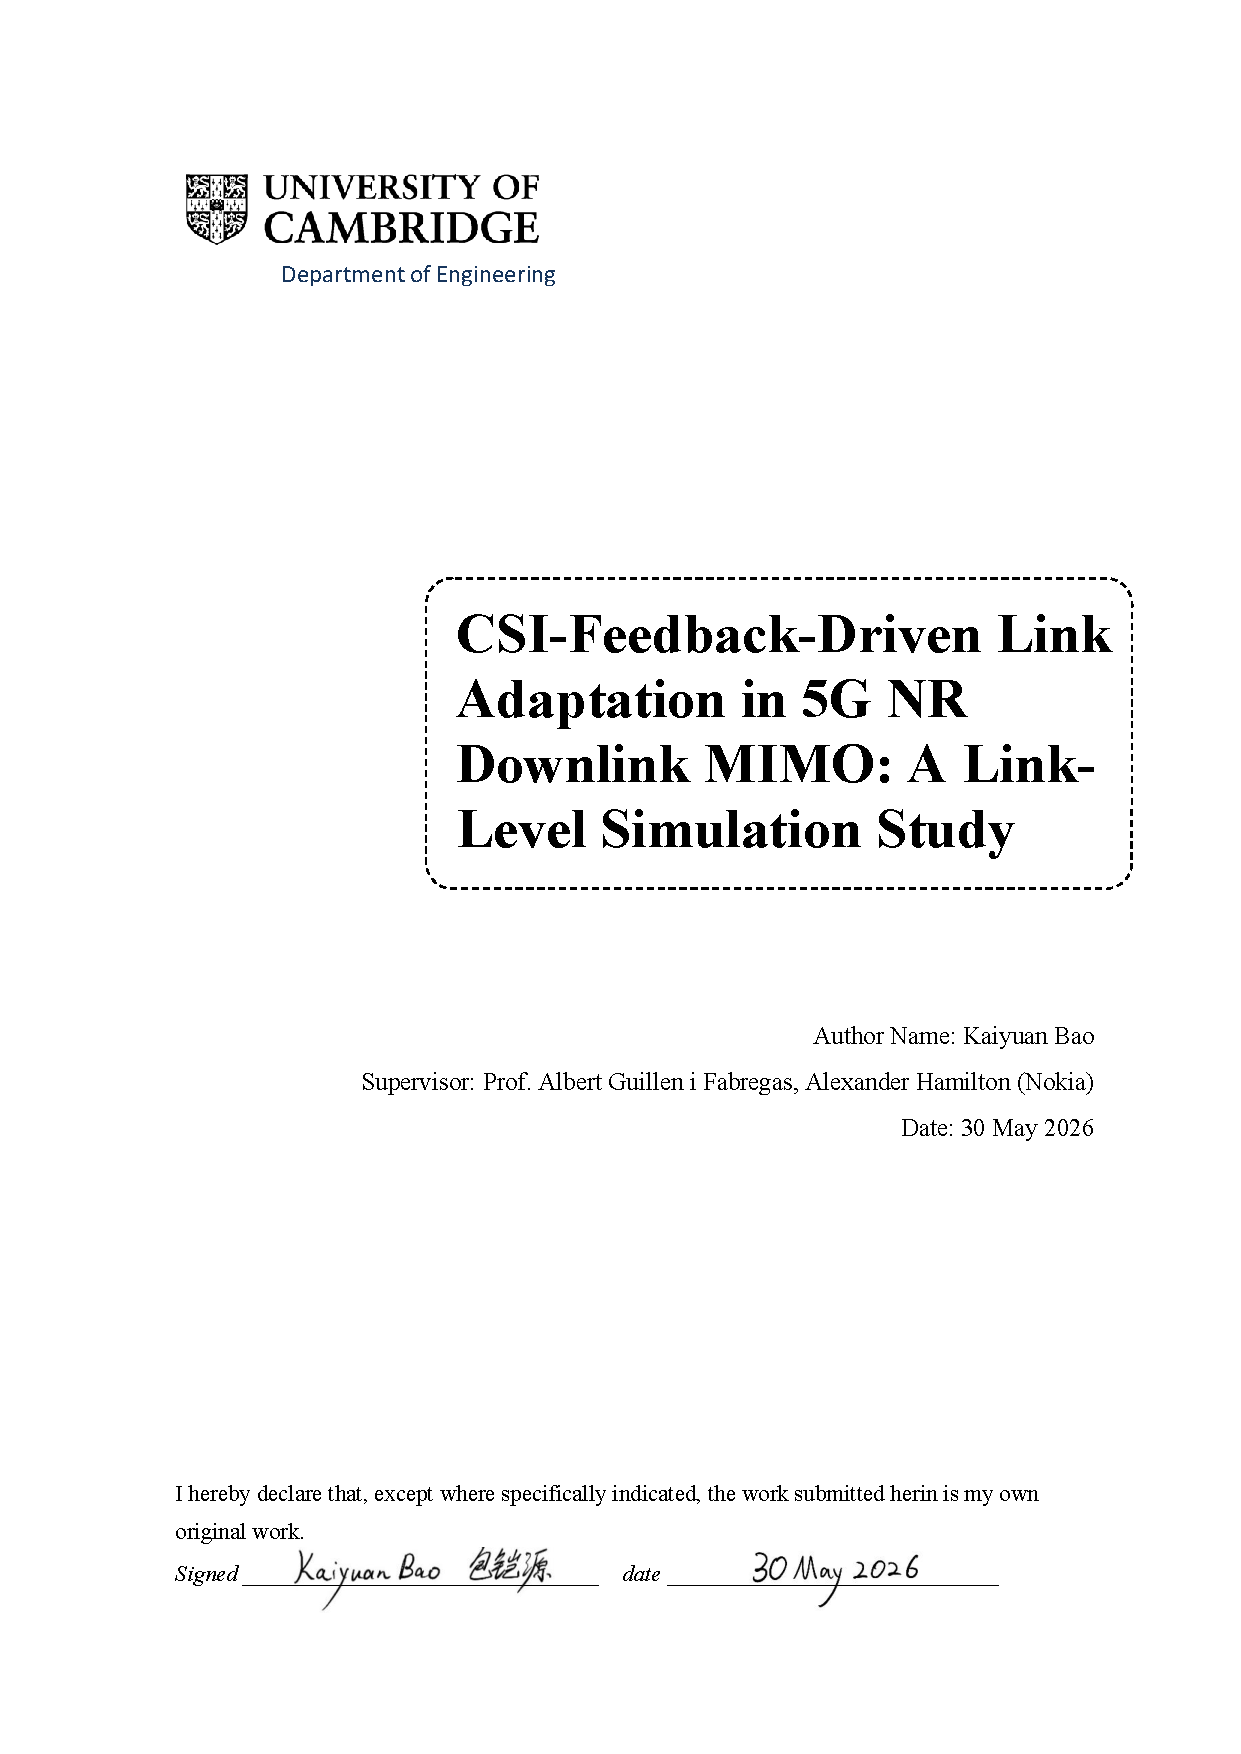
\includepdf[
	pages=1,
	pagecommand={\thispagestyle{empty}},
	fitpaper=true
	]{FrontPage.pdf}
\clearpage

\setcounter{page}{1}
\newpage
\section*{\centering Acknowledgement}
	This research project was completed under the direct supervision of Prof. Albert Guillen i Fabregas from the Department of Engineering, University of Cambridge, and Alexander Hamilton from Nokia. I sincerely thank them for their supervision, support, and encouragement throughout the year, as well as for their guidance on this project. \\
	\newline 
	The completion of this project marks the end of my four-year study at Cambridge. I would like to take this opportunity to thank my parents for their tremendous support during my years in the UK, which made it possible for me to pursue my studies at Cambridge.

\begin{flushright}
	Kaiyuan Bao \\ May 2026
	\end{flushright}

\newpage



	\maketitle
	\vspace{-35pt}
	\pagestyle{fancy}
	\fancyhead[L]{}   % 左侧页眉
	\fancyhead[C]{} 
	\fancyhead[R]{\rightmark}
	\renewcommand{\subsectionmark}[1]{\markright{#1}}  % 只显示标题，不显示编号
	
\thispagestyle{empty}
\section*{Background and Motivation}

\section*{Methodology}

\newpage

\thispagestyle{empty}
\section*{Key Results and Interpretation}

\section*{Conclusion}
	
\newpage
\tableofcontents
\thispagestyle{empty}
\newpage

\section*{List of Abbreviations}
\thispagestyle{empty}
\addcontentsline{toc}{section}{List of Abbreviations}

\begin{longtable}{p{3cm}p{10cm}}
	\textbf{Abbreviation} & \textbf{Definition} \\
	\hline
	
	3GPP    & Third Generation Partnership Project \\
	
	5G      & Fifth Generation \\
	
	BER     & Bit Error Rate \\
	BLER    & Block Error Rate \\
	
	CDL     & Clustered Delay Line \\
	CP      & Cyclic Prefix \\
	CQI     & Channel Quality Indicator \\
	CSI     & Channel State Information \\
	CSI-RS  & Channel State Information Reference Signal \\
	CW      & Codeword \\
	
	DL      & Downlink \\
	DM-RS   & Demodulation Reference Signal \\
	
	FR & Frequency Range \\
	
	gNB     & Next Generation Node B \\
	
	HARQ    & Hybrid Automatic Repeat Request \\
	
	LDPC    & Low-Density Parity-Check \\
	LOS     & Line-of-Sight \\
	
	MCS     & Modulation and Coding Scheme \\
	MIMO    & Multiple-Input Multiple-Output \\
	
	NLOS    & Non-Line-of-Sight \\
	NR      & New Radio \\
	NZP     & Non-Zero Power \\
	
	OFDM    & Orthogonal Frequency Division Multiplexing \\
	
	PDCCH   & Physical Downlink Control Channel \\
	PDSCH   & Physical Downlink Shared Channel \\
	PMI     & Precoding Matrix Indicator \\

	
	QAM     & Quadrature Amplitude Modulation \\
	QPSK    & Quadrature Phase Shift Keying \\
	
	RAN     & Radio Access Network \\
	RB      & Resource Block \\
	RE      & Resource Element \\
	RI      & Rank Indicator \\
	
	SCS     & Subcarrier Spacing \\
	SINR    & Signal-to-Interference-and-Noise Ratio \\
	SISO    & Single-Input Single-Output \\
	SNR     & Signal-to-Noise Ratio \\
	
	TB      & Transport Block \\
	TBS     & Transport Block Size \\
	TCR     & Target Code Rate \\
	TDL     & Tapped Delay Line \\
	
	UE      & User Equipment \\
	UL      & Uplink \\
	UMa &  Urban Macrocell \\
	UMi & Urban Microcell \\
	
	XPR & cross polarization power ratios \\
	
\end{longtable}
\newpage

\section{Introduction}
\subsection{Motivation and Project Scope}
\begin{highlightblock} 
	Mobile telecommunications have experienced rapid development over the past three decades. The second-generation (2G) mobile systems represented a major milestone in the history of mobile communications, ???as they enabled the large-scale adoption of mobile phones for voice and text services. Although 2G was not primarily designed for high-rate data transmission, it established mobile communication as a mass-market technology and introduced early forms of digital data services. ??? Subsequent generations then progressively improved the capability of mobile networks to support packet data transmission. Third-generation (3G) systems enabled more practical mobile internet access, while fourth-generation long-term evolution (4G LTE)in the early 2010s provided substantially higher data rates and lower latency, making services such as video streaming, mobile applications, and real-time online communication widely accessible to end users.
	
	The evolution from 3G to 4G and 5G has been enabled by a combination of physical-layer and system-level innovations. These include the adoption of orthogonal frequency division multiple access (OFDMA), more advanced channel coding and modulation schemes, adaptive link adaptation, and increasingly sophisticated multi-antenna transmission techniques \cite{Manikas}. In particular, the use of multiple-input multiple-output (MIMO) techniques has become increasingly important as mobile networks have moved towards higher data rates, and more reliable wireless links. Rather than relying only on additional bandwidth or higher transmit power, MIMO systems exploit the spatial dimension of the wireless channel by using multiple transmit and receive antennas.
\end{highlightblock}

\begin{highlightblock}
	Building upon the capabilities of 4G LTE, the fifth-generation mobile communication system, known as 5G New Radio (5G NR), has been designed to support a wide range of service requirements. Three main usage scenarios are commonly associated with 5G: enhanced mobile broadband (eMBB), massive machine-type communications (mMTC), and ultra-reliable and low-latency communications (URLLC) \cite{EricssonBook}. These scenarios impose different and sometimes competing requirements on the radio access network, including high peak data rates, high spectral efficiency, massive device connectivity, low latency, and high reliability. 
\end{highlightblock}

\begin{highlightblock}
	MIMO plays a central role in meeting these requirements in 5G NR. By transmitting multiple spatial layers over the same time-frequency resources, spatial multiplexing can significantly increase throughput when the wireless channel supports multiple spatial paths. Beamforming can also be used to direct transmitted energy towards the intended user, improving the received signal quality and reducing interference. In larger antenna-array systems, often referred to as massive MIMO, these benefits can be further enhanced \cite{Ericsson_MIMO}. However, the achievable gain from the system is highly dependent on factors such as the antenna configuration, the selected number of layers, the modulation and coding scheme, and the accuracy of the channel information available at the transmitter.
\end{highlightblock}

\begin{highlightblock}
	This project focuses specifically on channel-state-information (CSI) feedback for downlink MIMO transmission in 5G NR. In a practical feedback-based downlink system, the base station does not have perfect and instantaneous knowledge of the downlink channel. Instead, the user equipment (UE) estimates the channel using reference signals and reports quantised CSI information back to the base station. This CSI feedback is then used to support link adaptation and MIMO transmission decisions. In 5G NR, the reported CSI may include the channel quality indicator (CQI), rank indicator (RI), and precoding matrix indicator (PMI). These quantities are closely related to the modulation and coding scheme, the number of spatial layers, and the precoder used for downlink data transmission.
\end{highlightblock}

\begin{highlightblock}
	The structure and configuration of CSI feedback therefore have a direct impact on system performance. For example, more detailed or more frequent CSI reporting can allow the transmitter to make better-informed decisions, especially when the channel varies rapidly. However, these improvements are not free. CSI-RS and feedback reporting consume downlink and uplink resources, respectively, thereby increasing system overhead and potentially introducing additional processing requirements at both the transmitter and receiver sides. Moreover, more detailed or denser feedback does not always translate into higher throughput, and may instead provide little practical benefit when the additional information cannot be effectively exploited by the system. This creates a trade-off between CSI feedback granularity, feedback overhead, channel variation, and achievable downlink performance.
\end{highlightblock}

\begin{highlightblock}
	The aim of this research project is to investigate how MIMO-related configurations and CSI feedback affect the throughput performance of 5G NR downlink. The study is simulation-based and focuses on the interaction between CSI reporting and link adaptation. In particular, the project examines how different antenna configurations, channel models and CSI reporting periodicity influence the resulting throughput and the overall performance of the system. These parameters are studied under representative channel and mobility conditions in order to reach a balance in the trade-offs under different scenarios.

\end{highlightblock}

\begin{highlightblock}
	The Third Generation Partnership Project (3GPP) provides the global standardisation framework for mobile communication systems. Originally established for the development of third-generation cellular specifications, its scope has since expanded to cover the continuous evolution of LTE, 5G NR, 5G-Advanced, and future technologies beyond 5G. 5G NR was first introduced through 3GPP Release~15, which defined the first phase of the 5G system and provided the basis for practical 5G deployment. Subsequent releases have continued to enhance the 5G system, with Release~18 and Release~19 forming part of the 5G-Advanced evolution. Future releases are expected to provide the basis for the transition towards 6G \cite{3GPP}.
	
	The simulations in this project are conducted in MATLAB using a framework aligned with relevant 3GPP specifications. This alignment includes the use of standardised channel models, such as CDL models, as well as representative baseline system parameters commonly adopted in 5G NR link-level studies, including carrier frequency, bandwidth, subcarrier spacing, antenna configuration, and reference signal structure. The research project sims to provide insights that can support future 3GPP standardisation discussions related to MIMO techniques in 5G and 6G. 
\end{highlightblock}

\subsection{Report Structure}

\begin{highlightblock}
	The remainder of this report is organised as follows. Section~2 presents the background and methodology of the project. It first introduces the 5G NR downlink physical layer, followed by the overall transmission framework and CSI feedback mechanism. The channel models, Doppler shift are then introduced, followed by the overview of the simulation framework, and the adopted system configuration.
	
	Section~3 focuses on model validation and the introduction of baseline CSI-feedback-driven downlink behaviour. The model is validated by comparing the BLER curve with the results reported by other companies under fixed-MCS transmission. Then the results for the baseline CDL-C \(4 \times 4\) throughput behaviour with CSI-feedback is presented. The CSI-driven link adaptation statistics are also investigated in depth to understand the baseline behaviour. 
	
	Section~4 investigates the robustness of the observed behaviour across different MIMO and channel configurations. This includes an antenna configuration sweep, a CDL channel profile sweep, and one-layer control experiments, allowing the sensitivity of the system performance to spatial and channel conditions to be assessed.
	
	Section~5 forms the central CSI-focused part of the report, studying how mobility and CSI reporting periodicity affect the effectiveness of CSI-feedback-driven link adaptation. It compares different CSI reporting periodicities under different mobility conditions, in order to examine whether more frequent CSI updates can improve the transmitter's adaptation decisions and increase downlink throughput. The section concludes by discussing the practical trade-off between CSI freshness, reporting overhead, and throughput gain. This provides the main basis for evaluating when denser CSI feedback is beneficial, and when the additional feedback cost is not justified.
	
	Section~6 provides the final discussion and conclusion. It interprets the main simulation results, discusses the limitations of the study, outlines possible future work, and summarises the implications for 5G NR and future wireless systems. 
	
	The references are listed in Section~7 and the supporting information are presented in Section~8 appendix.
\end{highlightblock}

\section{Background and Methodology}
\label{sec:2}
\subsection{5G NR Downlink Physical Layer Overview}
\hl{
	1. OFDM\\
	2. PDSCH (DL)\\
	3. DM-RS\\
	4. CSI-RS\\
	5. Slot, RB\\
	6. Definition of BER/BLER/Throughput\\
	7. Why throughput not BER}
	\newpage
	
\subsection{MIMO Transmission and CSI Feedback}
	Specifics of CSI: PMI,RI, CQI \\
	Feedback loops\\
	How the modulation scheme/TCR/rank changes based on the feedback
	\begin{figure}[H]
		\centering
		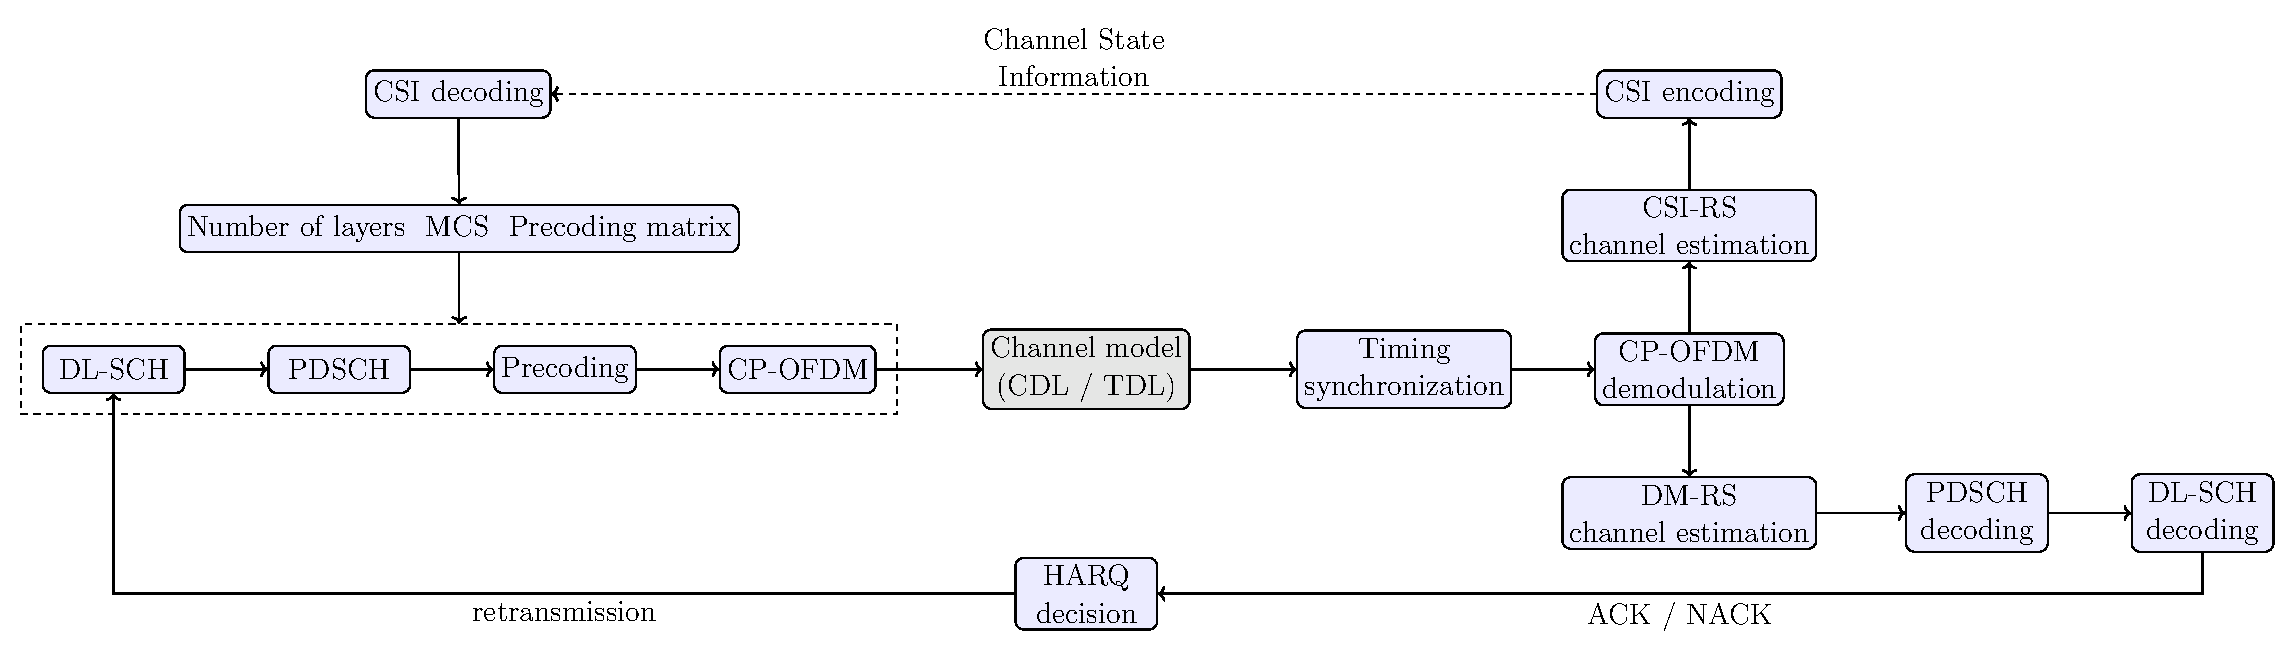
\includegraphics[width=1\linewidth]{figures/TIKZ_graph_1.pdf}
		\caption{Overview of the CSI-based downlink transmission and feedback framework, adapted from~\cite{Matlab_PDSCH_CSI}}
		\label{fig:csi_overview}
	\end{figure}
	
	\begin{highlightblock}
			[Not complete]
		As illustrated in Figure~\ref{fig:csi_overview}, the downlink transmission relies on channel state information (CSI) obtained through reference signal measurements at the receiver. The user equipment (UE) estimates the downlink channel based on CSI reference signals (CSI-RS). Based on the estimated channel, the CSI is encoded into three main feedback components: the Channel Quality Indicator (CQI), Precoding Matrix Indicator (PMI), and Rank Indicator (RI).
		
		CQI is a 4-bit indicator with values ranging from 0 to 15, representing the reported downlink channel quality. It provides an indication of the highest modulation scheme and coding rate that can be supported under a predefined target block error rate (BLER). The precoding matrix indicator (PMI) specifies the precoding matrix applied at the transmitter, while the rank indicator (RI) indicates the recommended number of transmission layers \cite{Matlab_PDSCH_CSI}.
		
		There are various parameters that affect the quality of the CSI. These include the CSI reporting periodicity, which controls how frequently the feedback is updated, as well as the reporting mode, which can be configured as wideband or subband. In addition, parameters such as the codebook type and mode, and the subband size further impact the granularity of the reported CSI. In time-varying channels, infrequent or coarse CSI reporting may lead to outdated channel knowledge at the transmitter, therefore degrading the performance of the transmission.
	\end{highlightblock}
	\begin{highlightblock}	
		The reported CSI is fed back to the transmitter and used to configure key downlink transmission parameters, including the modulation scheme, target code rate, number of transmission layers, and the precoding matrix. Using these updated parameters, the transmitter processes the data through the DL-SCH and maps it to the PDSCH, followed by precoding and CP-OFDM modulation before transmission over the wireless channel. At the receiver, the received signal is synchronised, demodulated, and decoded using demodulation reference signals (DM-RS) for coherent detection.
			\end{highlightblock}
		

\subsection{CDL Channel Model and Doppler Shift}
\hl{
	CDL model definition\\
	CDL ABCDE difference, why CDL-C default\\
	Doppler shift definition and impact\\
	
	Also: Why demodulation performance, cdl more realistic, not just TDL to verify if everything works, ....}
	\begin{highlightblock}	
			[Not complete]
		There are two widely used channel models in 5G NR link-level evaluations, namely the tapped delay line (TDL) model and the clustered delay line (CDL) model. Each model has several variants designed to represent different propagation environments such as urban, suburban, and rural scenarios. The TDL model provides a simplified representation of the multipath channel and is commonly used for baseline evaluations or scenarios where spatial characteristics and multi-antenna effects are not modelled.
		
		
		
		In the TDL model, the channel is represented as a superposition of multiple discrete propagation paths (taps), each characterised by a specific delay $\tau_l$ and a path gain $h_l(t)$:
		\begin{equation}
			h(t, \tau)=\sum_{l=0}^{L-1}h_l(t)\delta(\tau-\tau_l).
		\end{equation}
		The TDL model does not represent angular or spatial features of the propagation channel. In contrast, the clustered delay line (CDL) model incorporates spatial information and therefore provides a more realistic channel description. Similar to the TDL model, the CDL model defines a set of multipath clusters characterised by relative delays and average powers. In addition, each cluster is associated with angular parameters, including the azimuth and zenith angles of departure and arrival (AoD, AoA, ZoD, and ZoA). Each cluster is further decomposed into multiple sub-rays with random initial phases and Doppler components. By modelling these spatial characteristics, the CDL channel model enables a more accurate representation of the spatial characteristics of MIMO channels, at the cost of increased complexity and higher computational cost \cite{ETSI_TDL_CDL}.
		
				The CDL profiles are defined by their cluster-level delay, power, angular parameters, angular spreads and XPR. 
				
		In addition to CSI, 5G NR also employs hybrid automatic repeat request (HARQ) to improve the robustness of the transmission through re-transmissions. After DL-SCH decoding at the receiver, an acknowledge/negative acknowledge (ACK/NACK) signal is fed back to the transmitter, which indicates whether a re-transmission is required. In the case of a decoding failure, the transport block is re-transmitted using a different redundancy version (RV) and combined at the receiver, thus increasing the probability of successful decoding \cite{EricssonBook} \cite{MathWorks2026}.
	\end{highlightblock}
		
	
\begin{table}[H]
	\centering
	\caption{Summary of CDL channel model profiles based on 3GPP TR 38.901 \cite{3GPP2026}}
	\label{tab:cdl_models}
	
	\renewcommand{\arraystretch}{1.15}
	\begin{tabularx}{\textwidth}{@{} l c >{\raggedright\arraybackslash}X c @{}}
		\toprule
		\textbf{\makecell{Channel \\ Model}} 
		& \textbf{LOS/NLOS} 
		& \textbf{Characteristics} 
		& \textbf{\makecell{Indicative \\ Use Case$^\dagger$}} \\
		\midrule
		CDL-A 
		& NLOS 
		& Profile with relatively limited angular dispersion compared with CDL-B, and a higher XPR than CDL-B/C. 
		& UMi \\
		
		CDL-B 
		& NLOS 
		& Profile with the largest azimuth angular spread among the NLOS CDL profiles. 
		& UMi \\
		
		CDL-C 
		& NLOS 
		& Profile with a richer delayed multipath structure, more clusters, and the smallest departure angular spread among the NLOS CDL profiles. 
		& UMa \\
		
		CDL-D 
		& LOS 
		& Profile including a specular LOS component. 
		& UMa \\
		
		CDL-E 
		& LOS 
		& Profile including a specular LOS component, with a longer normalised delay tail than CDL-D. 
		& UMa \\
		\bottomrule
	\end{tabularx}
	
	\vspace{0.5em}
	\begin{minipage}{\textwidth}
		\footnotesize
		$^\dagger$ The indicated use cases are interpretative examples rather than fixed definitions in 3GPP TR 38.901. 

		Their association with UMi or UMa scenarios depends on the selected RMS delay spread and the overall simulation setup.
	\end{minipage}
\end{table}
	
\subsection{MATLAB Simulation Framework}
\begin{highlightblock}
	
	
	The project is carried out using MATLAB and its 5G Toolbox, with a simulation framework aligned with relevant 3GPP specifications. This alignment includes the use of standardised channel models, such as clustered delay line (CDL) models, and representative system parameters commonly used in 5G NR link-level studies, including carrier frequency, bandwidth, subcarrier spacing, antenna configuration, and reference signal structure. The use of a 3GPP-aligned simulation framework allows the results to be interpreted in the context of practical 5G NR physical-layer design, while still providing sufficient flexibility to isolate the effects of individual CSI and MIMO parameters.
	

\end{highlightblock}

	\begin{highlightblock}
		Table~\ref{tab:system_config} below summarises the baseline system and channel configuration adopted in this study, which is aligned with the assumptions commonly used in 3GPP evaluation studies, including TR~38.753~\cite{3GPPSimulationSpec}. The full set of parameters used are shown in the Appendix section Table \ref{tab:appendix1}. There different mobility scenarios are considered. The low-mobility case assumes a maximum Doppler shift of 10~Hz, corresponding to a UE speed of 3 km/h, a default setting for 3GPP testing. For medium- and high-mobility cases, the 100~Hz and 390~Hz Doppler shift corresponds to the speed of approximately 30~km/h and 120~km/h respectively for a 3.5 GHz carrier frequency.
	\end{highlightblock}

		
		\begin{table}[H]
			\centering
			\caption{System and channel configuration used in the simulations}
			\label{tab:system_config}
			\begin{tabular}{ll}
				\hline
				\textbf{Parameter} & \textbf{Value} \\
				\toprule
				Carrier frequency      & FR1, 3.5 GHz \\
				Subcarrier spacing          & 30 kHz \\
				Channel bandwidth           & 106 RBs \\
				Antenna configuration       & 4 Tx, 4 Rx \\
				Maximum number of layers    & 4 \\
				Channel model               & CDL-C \\
				Mobility scenarios          & \makecell[l]{10~Hz (Default), 100~Hz, 390~Hz}\\
				Simulation type             & Downlink link-level \\
				\hline
			\end{tabular}
		\end{table}
		
		
		\begin{highlightblock}
			The CDL-C channel model is selected as it represents a typical non-line-of-sight (NLOS) urban macro environment and is widely used in 3GPP evaluation studies, while modelling spatial characteristics are essential for the study of CSI feedback. A 4$\times$4 MIMO configuration with up to four transmission layers is considered, reflecting a representative frequency range 1 (FR1) deployment while maintaining a manageable simulation complexity. This configuration allows multi-layer transmission as well as rank adaptation to be studied within a single-codeword framework, avoiding additional variability introduced by using an additional codeword, and thus enabling a clearer assessment of the effect of the CSI feedback parameters.
			
		\end{highlightblock}
		
		\begin{highlightblock}
		The PDSCH, DM-RS and CSI-RS parameters used for the downlink resource-grid illustration are summarised in Table~\ref{tab:dl_grid}. Based on these configurations, the downlink resource grid is shown in Fig.~\ref{fig:24ResouceGrid} for a CSI-RS-active slot. The first two OFDM symbols are left unallocated because the PDSCH time-domain allocation starts from symbol 2. In practice, these initial symbols can be reserved for downlink control signalling, such as PDCCH transmission within a CORESET, although PDCCH is not explicitly modelled in this link-level simulation.
			
		\end{highlightblock}
		
			\begin{table}[H]
				\centering
					
				\caption{Key PDSCH, DM-RS and CSI-RS parameters used for simulation}
				\label{tab:dl_grid}
				\begin{tabular}{|ll|c|}
				\hline
				\multicolumn{2}{|c|}{\textbf{Parameter}}                                                                                                                                   & \textbf{Value}               \\ \hline
				

				\multicolumn{1}{|l|}{\multirow{4}{*}{PDSCH configuration}}      & Mapping type                                                                                    & Type A              \\ \cline{2-3} 

				\multicolumn{1}{|l|}{}                                          & Starting symbol                                                                                 & 2                   \\ \cline{2-3} 
				\multicolumn{1}{|l|}{}                                          & Length                                                                                          & 12                  \\ \hline
				\multicolumn{1}{|c|}{\multirow{5}{*}{PDSCH DMRS configuration}} & DMRS Type                                                                                       & Type 1              \\ \cline{2-3} 
				\multicolumn{1}{|c|}{}                                          & Number of additional DMRS                                                                       & 1                   \\ \cline{2-3} 
				\multicolumn{1}{|c|}{}                                          & \begin{tabular}[c]{@{}l@{}}Max. number of OFDM \\ symbols for DL front loaded DMRS\end{tabular} & 2                   \\\cline{2-3} 
				
				\multicolumn{1}{|c|}{} & Number of CDM groups without data & 1  \\ \cline{2-3} 
				
				
				 \hline 
				
				\multicolumn{1}{|l|}{\multirow{4}{*}{\begin{tabular}[c]{@{}l@{}}NZP CSI-RS for \\ CSI acquisition\end{tabular}}} & CSI-RS resource type       &       Periodic \\ \cline{2-3} 
				\multicolumn{1}{|l|}{}                                                                                           & Density                          & 1        \\ \cline{2-3} 
				
				\multicolumn{1}{|l|}{}                                                                                           & Symbol location                         & 4        \\  \cline{2-3} 
				\multicolumn{1}{|l|}{}                                                                                           & Subcarrier location                         & 0        \\ \cline{2-3} 
			 \hline 
				
			\end{tabular}
			\end{table}

		\begin{figure}[H]
			\centering
			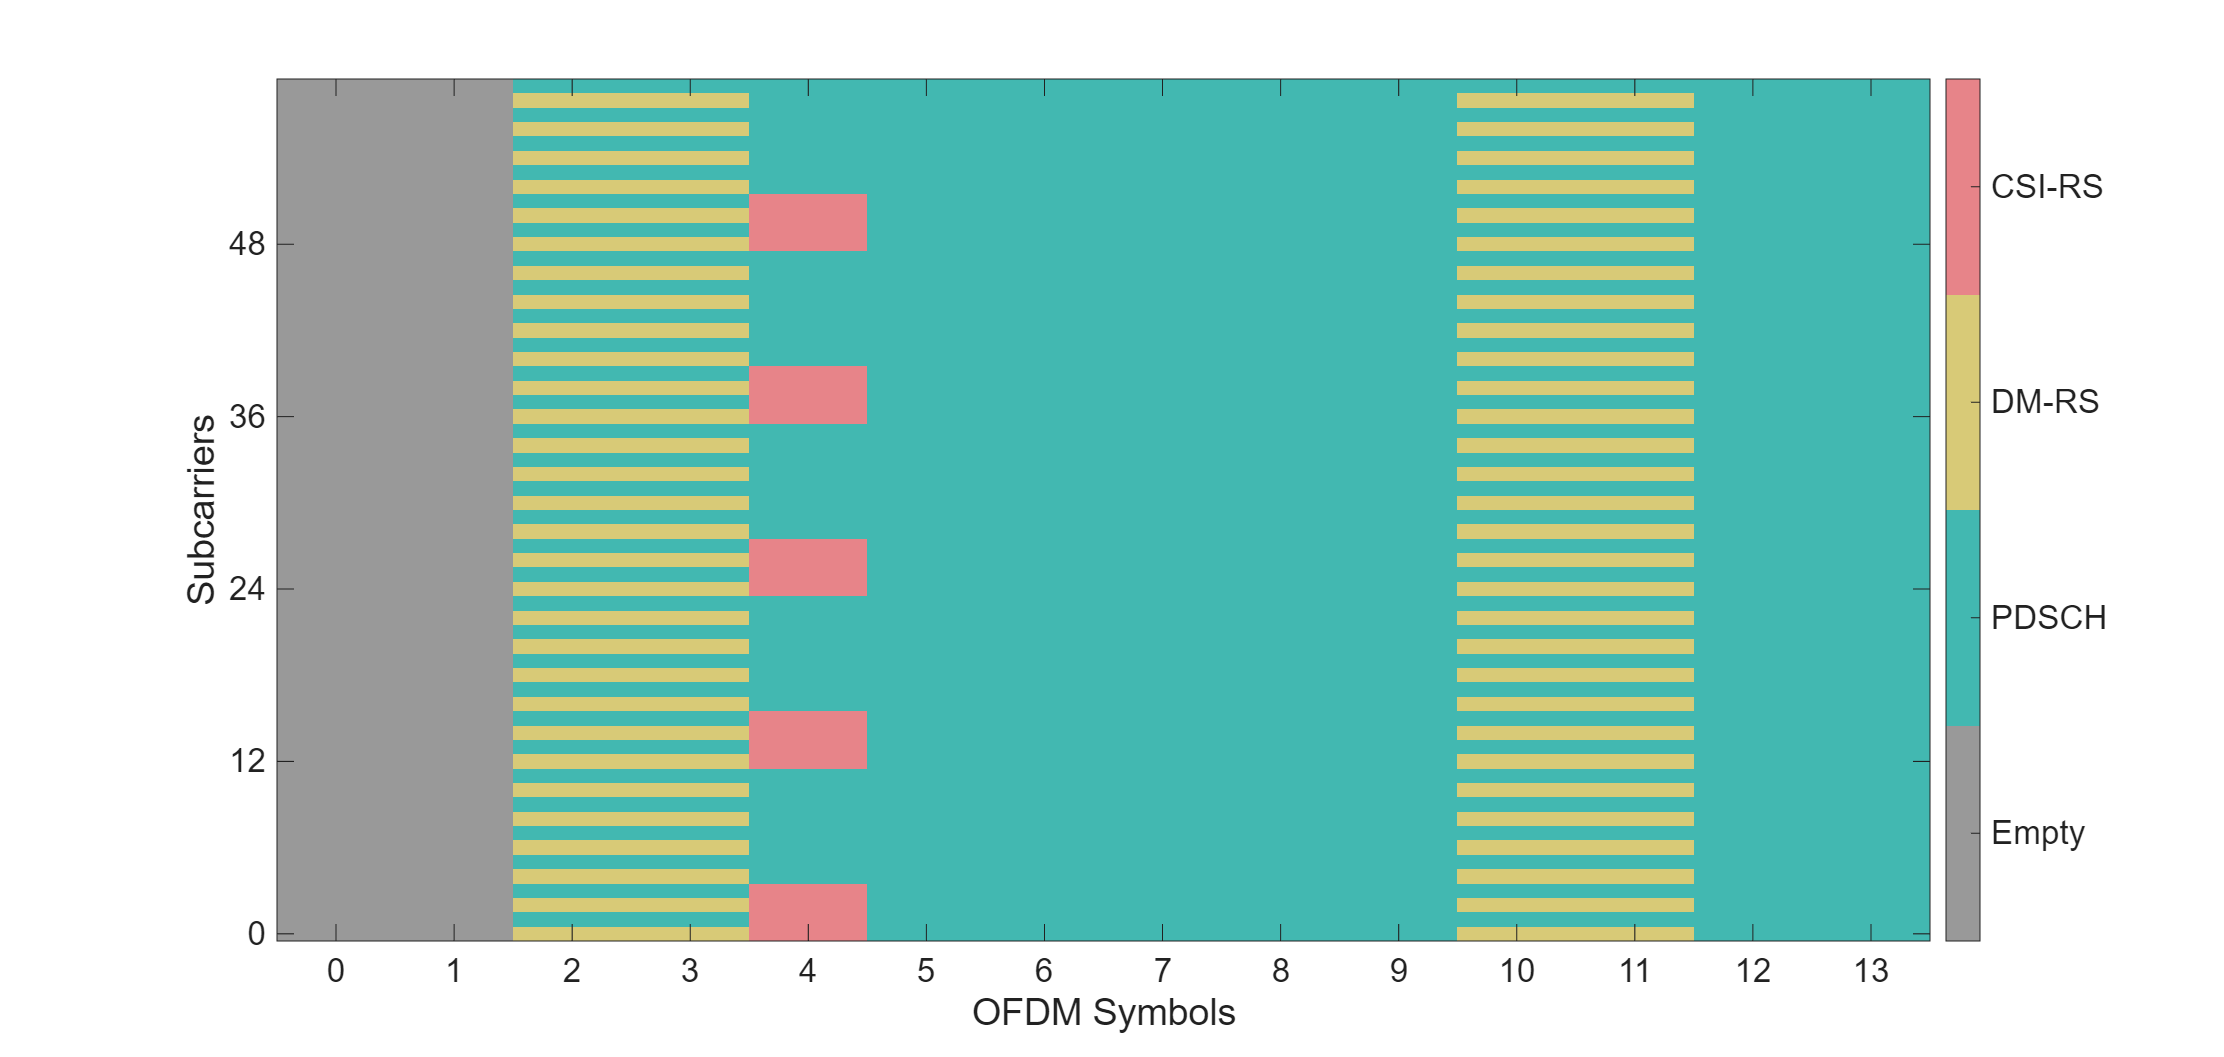
\includegraphics[width=\linewidth]{figures/24ResouceGrid.png}
			\caption{Downlink resource grid showing the allocation of PDSCH, DM-RS and CSI-RS}
			\label{fig:24ResouceGrid}
		\end{figure}
	\subsection{System Configuration and Experimental Design}
		\begin{highlightblock}
			This study focuses on investigating the impact of CSI feedback parameters on downlink transmission performance. The baseline CSI configuration follows the settings specified in relevant 3GPP specifications, including TS~38.101-4~\cite{3gpp_ts_38101_4}. Both the baseline configuration and the investigated parameter ranges are summarised in Table~\ref{tab:csi_config}. The investigated ranges represent the set of valid discrete configurations specified by 3GPP. Unless otherwise stated, all simulations use the baseline CSI configuration listed in Table~\ref{tab:csi_config}. The full set of CSI configurations used are shown in the Appendix section Table \ref{tab:appendix2}.
		\end{highlightblock}

		\begin{table}[H]
			\centering
			\caption{Baseline CSI feedback configuration used in the simulation framework}
			\label{tab:csi_config}
			\begin{tabular}{ll}
				\hline
				\textbf{Parameter} & \textbf{Baseline setting}  \\
				\toprule
				CSI report periodicity      & 10 slots \\
				CQI reporting mode          & Wideband  \\
				PMI reporting mode          & Wideband  \\
				Subband size                & 16 RBs   \\
				RI configuration            & Adaptive \\
				Codebook type               & Type I    \\
				Codebook mode               & Mode 1   \\
				\hline
			\end{tabular}
		\end{table}
		
		
	\begin{highlightblock}
		In section \ref{sec:3}, the behaviour of the system under baseline condition will be simulated and investigated. In section \ref{sec:4}, the performance of the system under different MIMO, CDL channel configurations will be investigated, which examines whether the baseline behaviour observed in the baseline scenario remains interpretable under these changes. In section \ref{sec:5}, the CSI reporting period will be varied to analyze suitable reporting period for different scenarios and the underlying reasons behind the observations. 
		
		Only a subset of the parameters under investigation is varied in each experiment, while the remaining parameters are kept fixed at their baseline values to ensure a controlled comparison. Table \ref{tab:sim_studies} shows a brief summary of the simulation study groups that are going to be simulated. <Note that sometimes may change multiple parameters at the same time..>
	\end{highlightblock}
	
	
	\begin{table}[H]
		\centering
		\caption{Summary of simulation study groups and objectives}
		\label{tab:sim_studies}
		\small
		\setlength{\tabcolsep}{5pt}
		\renewcommand{\arraystretch}{1.12}
		\begin{tabularx}{0.95\textwidth}{
				>{\raggedright\arraybackslash}p{0.25\textwidth}
				>{\raggedright\arraybackslash}X
				>{\raggedright\arraybackslash}p{0.30\textwidth}
			}
			\toprule
			\textbf{Study group} & \textbf{Purpose} & \textbf{Varied parameter} \\
			\midrule
			Baseline 
			& CDL-C \(4 \times 4\) reference performance 
			& -- \\
			
			Fixed-rank controls 
			& Layer adaptation 
			& RI \(=1\), RI \(\leq 2\), RI \(\leq 4\), \mbox{RI \(=4\)} \\
			
			MIMO configuration sweep 
			& Antenna configuration sensitivity 
			& \(2 \times 2\), \(4 \times 4\), \(8 \times 4\) \\
			
			CDL profile sweep 
			& Channel-model robustness 
			& CDL-B, CDL-C, CDL-D \\
			
			Doppler sweep 
			& Mobility sensitivity 
			& 10 Hz, 100 Hz, 390 Hz \\
			
			CSI period sweep 
			& CSI feedback freshness 
			& 4, 10, 64, 160 slots \\
			\bottomrule
		\end{tabularx}
	\end{table}
	
	\begin{table}[H]
		\centering
		\caption{Simulation execution settings}
		\label{tab:simulation_execution}
		\begin{tabular}{ll}
			\toprule
			\textbf{Parameter} & \textbf{Value} \\
			\midrule
			SNR range & $-5$ to $25$~dB, with 1~dB spacing \\
			Number of simulated frames & 1500 10-ms frames per SNR point \\
			Channel estimation & Practical channel estimation \\
			\bottomrule
		\end{tabular}
	\end{table}

\newpage
\section{Model Validation and Baseline CSI-Feedback Downlink Behaviour}
	\label{sec:3}
	
	
	\begin{highlightblock}
		At the beginning of the section, a simplified scenario where the adaption mechanism is temporarily disable, so that the modulation scheme, target code rate and number of transmission of layers are fixed is tested and compared with the results reported by other companies in the 3GPP technical reports. This is used to validate the correctness of the overall simulation framework.
		
		Afterwards, the CSI is enabled, andehe behaviour of the system under the baseline case as introduced in the last section is tested. The performance of the system as well as the role of CSI is investigated and analyzed in detail to provide a good understanding of the feedback decisions. At the second half of the section, a fixed-rank control is implemented to isolate the rank adaptation mechanism and .. the multi-layer transmission.
	\end{highlightblock}
	
	
	\subsection{External Link-Level Validation under Fixed-MCS Transmission}
	\begin{highlightblock}
	In the simulation model validation, a MCS 13 (Table 1), 4Tx 4Rx, 4-layer, random PMI transmission with a maximum Doppler of 10Hz setting is used. The HARQ is enabled in this simulation. The rest of the configurations remains unchanged from the default values defined in Table \ref{tab:system_config}. The modulation order, target code rate and number of PDSCH layers are fixed, so the result mainly reflects the decoding reliability of a given transmission. The performance is characterized by BLER. The plot is then compared with the simulated results reported by different firms, as shown in Fig. \ref{fig:31Validation}.  
	\end{highlightblock}
	
	\begin{highlightblock}
		The SNR corresponding to the 70\% and 30\% BLER is commonly used during comparison. The results are presented in the table below. 
	\end{highlightblock}

	\begin{figure}[H]
		\centering
		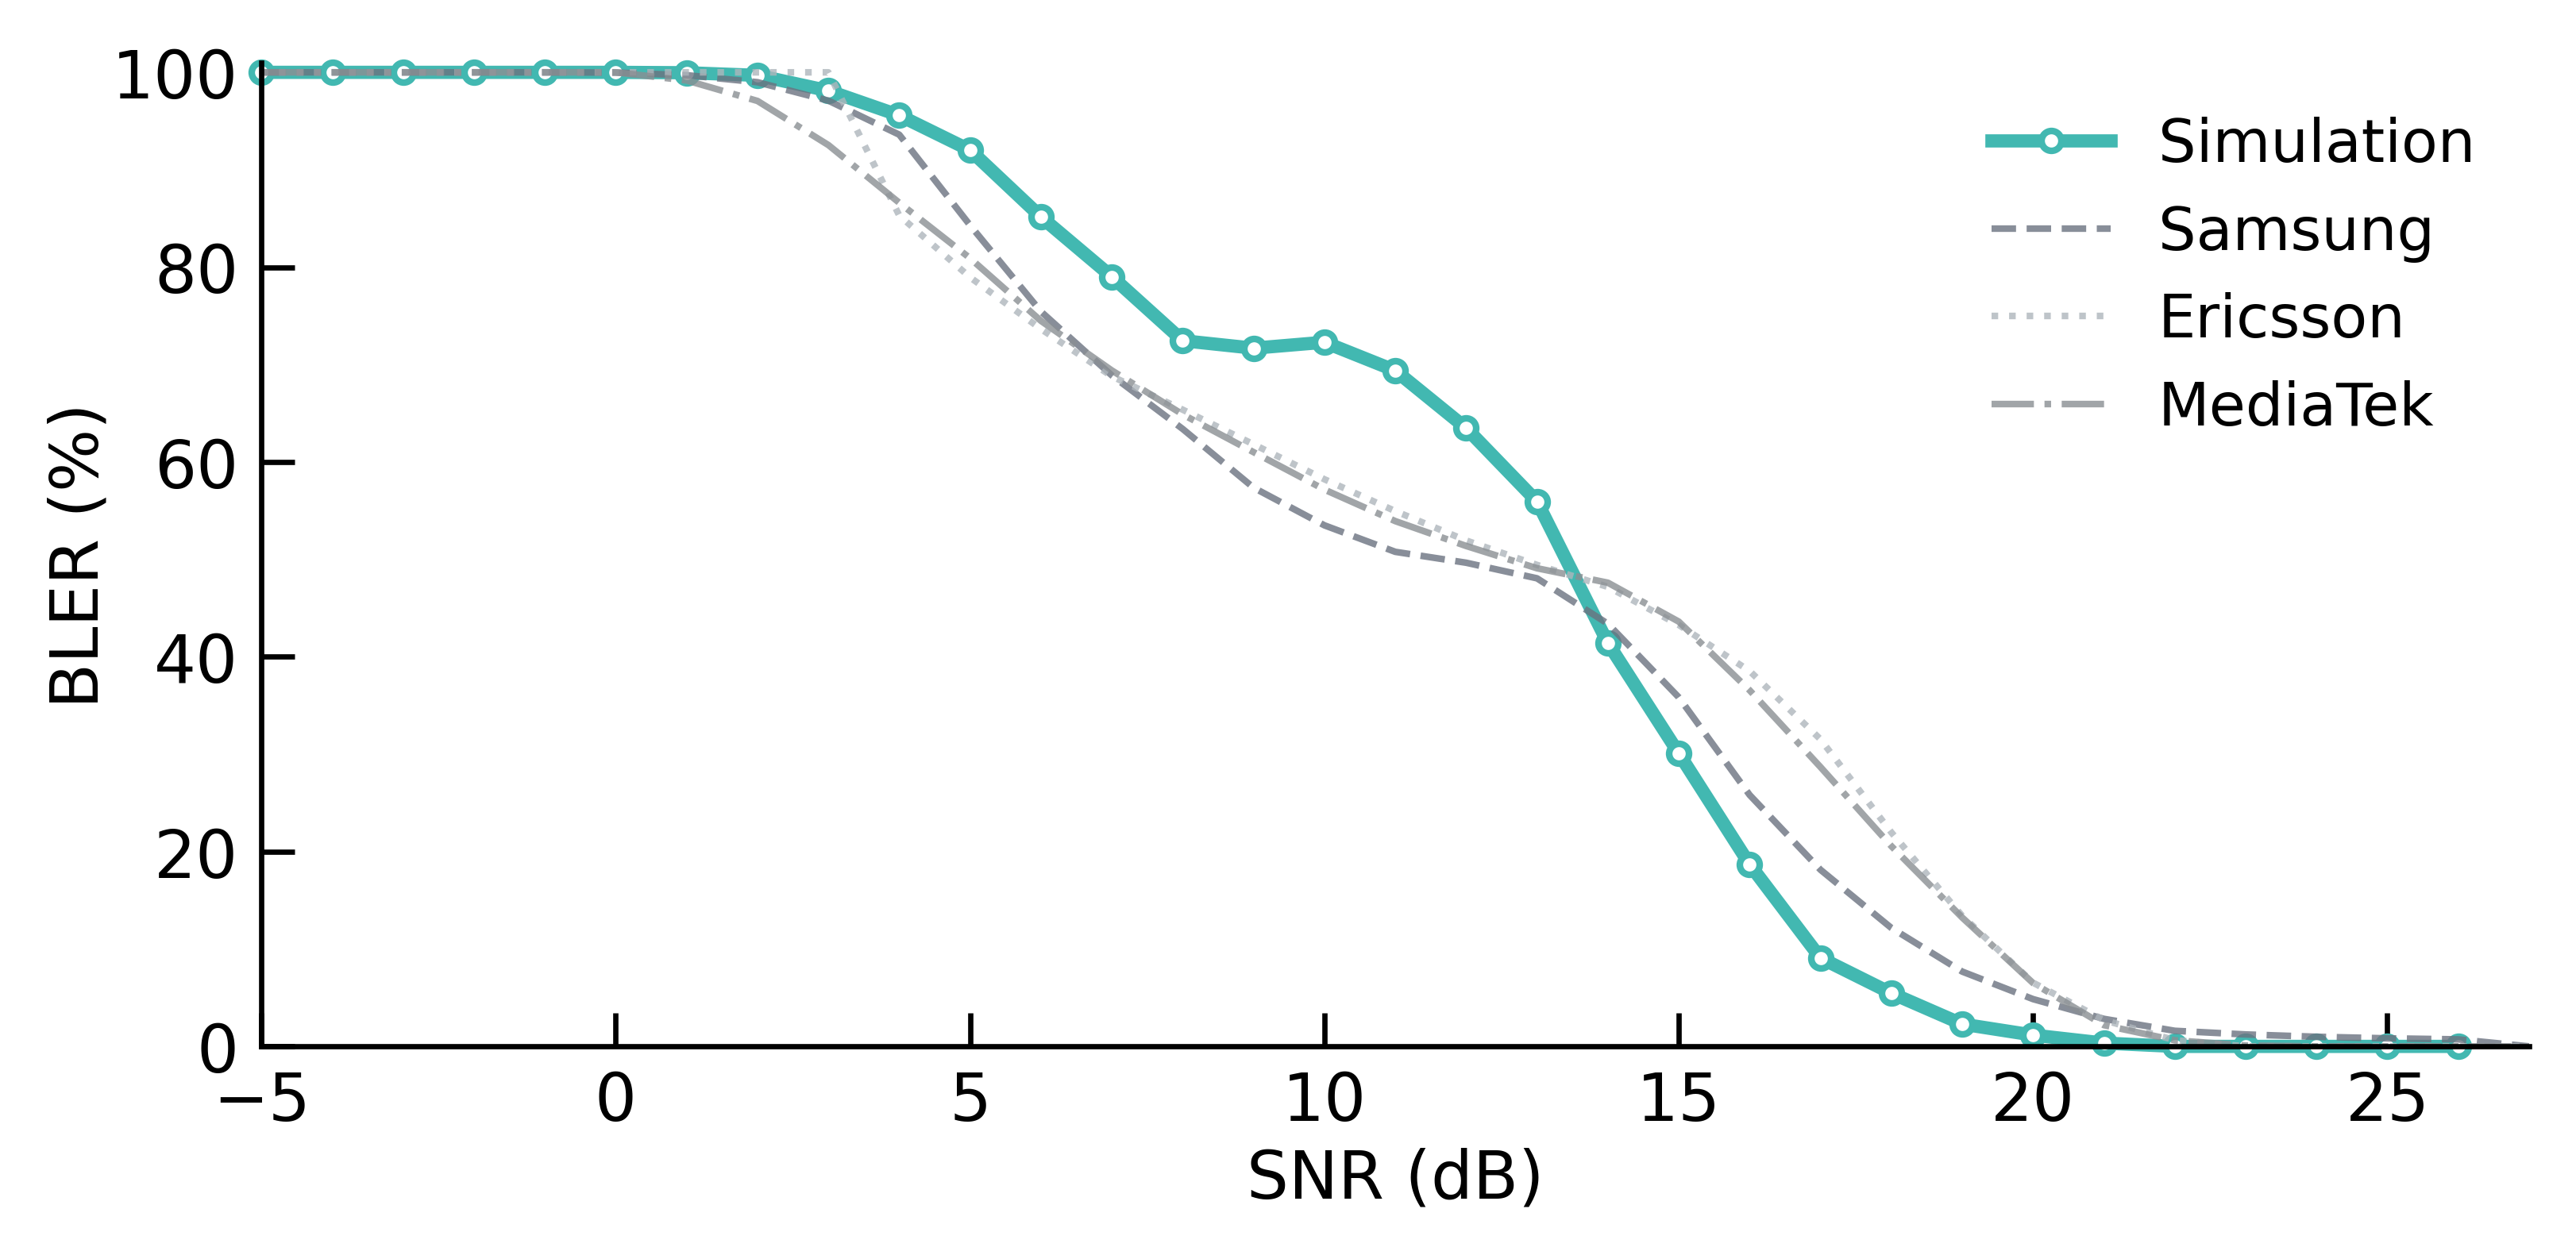
\includegraphics[width=0.75\linewidth]{figures/31Validation.png}
		\caption{BLER comparison between the simulation and firm-provided baselines, with firm data adapted from \cite{3gpp_ran4_results}}
		
		\label{fig:31Validation}
	\end{figure}
	
	
		\begin{table}[H]
		\centering
		\caption{Interpolated SNR required to achieve selected BLER levels for the simulation and firm-standard baselines}
		\label{tab:31}
				\begin{tabular}{cccccc}
			\midrule
			\textbf{\makecell{Target BLER\\(\%)}} & \textbf{Simulation} & \textbf{Samsung} & \textbf{Ericsson} & \textbf{MediaTek} & \textbf{Industry Average} \\
			\toprule
			70  & 10.8~dB&  6.8~dB & 6.8~dB  & 6.9~dB & 6.8~dB \\
			30  &  15.0~dB & 15.6~dB &17.2~dB  & 16.8~dB & 16.5~dB\\
			\bottomrule
		\end{tabular}
		
		\vspace{0.3em}
		\raggedright
		\footnotesize{$^\dagger$ SNR values obtained using linear interpolation.}
		
		\end{table}
	\begin{highlightblock}
		The simulated BLER curve follows the same general trend as the firm-provided baselines: the BLER remains close to 100\% at low SNR below 1~dB, decreases as the SNR increases, and approaches zero at high SNR above 23~dB. 
		
		From the simulated result, a plateau-like region is observed at intermediate SNR values, approximately between 7 and 10~dB. This behaviour may be partly attributed to the HARQ mechanism under the fixed-MCS configuration. Around 7~dB, the initial improvement in SNR allows some transport blocks that fail in the first transmission to be recovered through HARQ retransmission and combining, leading to a noticeable reduction in BLER. However, for the remaining more challenging channel realisations, the same fixed modulation, coding rate and layer configuration may still be too aggressive, so further BLER reduction is limited until the SNR becomes sufficiently high, above approximately 10~dB. Therefore, the plateau-like region can be interpreted as a transition region where HARQ improves the reliability of some blocks, but is not yet sufficient to recover the more difficult decoding cases.

	\end{highlightblock}
	\begin{highlightblock}
		The difference between the simulation and the firm-provided baselines is expected, as the comparison is not based on an identical receiver implementation. At 70\% BLER near the plateau, the discrepancy is around 4~dB, and at 30\% BLER, the discrepancy gets smaller to around 1.5~dB.
		
		Even with the same agreed transmission configuration, BLER is sensitive to implementation details such as channel estimation, LDPC decoding algorithm, iteration count, HARQ combining settings and so on. The specific details and the simulation files are not commonly disclosed by the firms, not to even say that the results obtained by the firms are likely to be conducted on the program constructed by the firms themselves, in stead of on public available software like MATLAB, or publicly available packages in Python. As a result, from the figure above, it is clear that large discrepancies around 2~dB even exist between the results of different firms.
		
 		As a result, it can be concluded that the simulated result in general aligns in a satisfactory manner with the industrial results. This validation should be interpreted as a qualitative and semi-quantitative alignment of the BLER trend, rather than an exact one-to-one reproduction of a specific BLER curve.
 		
	\end{highlightblock}
	\begin{highlightblock}
		For the subsequent simulation studies, throughput in Mbps is used instead of BLER as the main performance metric. This is because the later experiments involve CSI-driven link adaptation, where the MCS, number of layers and feedback configuration may change across transmission conditions. In such cases, the maximum achievable throughput will change every slot based on the settings, and therefore BLER alone is not sufficient to represent system performance. A configuration may achieve a low BLER simply by selecting a conservative MCS or fewer layers, but this does not necessarily imply high spectral efficiency or high user throughput. 
		
		Additionally, in real-life scenarios, the network operators generally focus more on the throughput than the BLER, as the throughput directly captures the useful successfully delivered data rate, which is what directly impacts the user experience. Therefore, throughput in Mbps is a more appropriate metric for comparing CSI-feedback and MIMO configurations in the rest of the project.
		
		Furthermore, HARQ was disabled in all subsequent simulation studies in order to isolate the impact of CSI feedback and MIMO-related configurations on the first-transmission performance. This also avoids introducing additional HARQ-related effects, such as the plateau-like behaviour observed in the fixed-MCS validation case discussed above. Since the objective of this project is to compare the relative impact of different CSI configurations rather than to optimise HARQ operation, disabling HARQ provides a cleaner and more controlled basis for comparison.
		
	\end{highlightblock}

	
	\subsection{Baseline CDL-C $4\times4$ Throughput Behaviour}
	\begin{highlightblock}
		Fig. \ref{fig:31StandardRun} presents the baseline downlink throughput for the CDL-C $4\times4$ MIMO configuration with adaptive CSI feedback. At the simulated range of -5~dB to 25dB, the throughput curve is increasing. The curve shows a gradual increase at low SNR, followed by a steeper transition region between approximately 5 dB and 17 dB. At 10dB, the throughput is approximately xxx Mbps. The throughput saturates at high SNR of approximately xxx Mbps. The bahaviour of the system is explained in the next subsection according to the CSI-related behaviours. This baseline provides the reference case against other scenarios compared in the subsequent simulations.
	\end{highlightblock}
		\begin{figure}[H]
			\centering
			
\includegraphics[width=0.75\linewidth]{figures/31StandardRun.pdf}
			\caption{Baseline downlink throughput performance for the CDL-C $4\times4$ configuration with adaptive CSI feedback}
			\label{fig:31StandardRun}
	\end{figure}
	
	\subsection{CSI-driven Link Adaptation Statistics}
	
	\begin{highlightblock}
	
		In addition to the performance of the system, the behaviour of the CSI during the transmission is shown in Fig. \ref{fig:32New_wMean} below. The four respective figures demonstrates the changes of CQI, target code rate (TCR), RI as the SNR changes as well as the use of modulation schemes at different SNR levels. CQI, TCR and RI are not fixed for each SNR testing point, but instead varies base on the real-time feedbacks and channel condition, even within subband (?). vertical bars which functions as the distribution spread indicator has been introduced to the three subfigures to characterize the consistency and variability. The bars indicate the 5th to 95th percentile range of each value range rather than the full minimum--maximum range. This choice is used to represent the typical spread of the selected CQI values while reducing the influence of rare extreme channel deep-fades or favorable fading realizations, making the results more representative.
		
		For CQI plot, as the SNR increases, the selected CQi rises gradually from 5 at low SNR to around 11 at high SNR, indicating that the link adaptation gets gradually more aggressive during the transmission due to the improved channel conditions. The peak CQI the system has every selected is 14. 
		
		Correspondingly, the target code rate of the system follows a similar trend, overall increasing from 0.4 to nearly 0.6 The TCR curve is not strictly increasing but instead having a oscillatory behaviour. The local minimum occur at SNR points where major change in modulation scheme occurs as the system would select a higher modulation scheme but in the meantime using a lower TCR. The two major local minimum occurs at around -3~dB and 4~dB, which corresponds to the SNR when the system switches the main modulation from QPSK to 16QAM, and from 16QAM to 64QAM respectively.
			\end{highlightblock}
			
			
		\begin{highlightblock}	

		The selected RI also changes with SNR, reflecting that the system changes the number of layers used for transmission under different channel conditions. At SNR lower than 2 dB, the system mainly selected RI = 1, representing a robust single-layer transmission. The RI increases to 2 at higher SNR, enabling steeper increase in throughput. Since the MIMO configuration is $4 \times 4$, a maximum of 4-layer transmission can be supported. However, the RI does not increase beyond 2 under this scenario, likely due to ...., partly causing the throughput to saturate to a throughput level below theoretical limit at very high SNR.
		
		For table 1 and 3 (...), three modulation schemes are supported, which are QPSK, 16QAM and 64QAM. 256 QAM is only supported when (...) and is uncommonly used due to its high requirement on channel condition. At very low SNR, the main modulation scheme is QPSK. As the SNR increases, QPSK quickly disappears and 16 QAM becomes dominant. For SNR higher than 10dB, 64QAM modulation dominates. The change in modulation scheme is gradual instead of abrupt, where the higher order modulation scheme will gradually be used more frequently as the SNR increases. The system uses 64 QAM for around 90\% of the cases, while the rest of the time using 16 QAM, likely during unusual channel degradation such as deep fade.
			\end{highlightblock}



	\begin{figure}[H]
		\centering
		
\includegraphics[width=1\linewidth]{figures/32New_wMean.pdf}
		\caption{CSI-driven link adaptation behaviour across SNR}
		\label{fig:32New_wMean}
	\end{figure}
	
		\begin{highlightblock}
			The shape of the throughput curve in Fig.~\ref{fig:31StandardRun} can be explained by the CSI-driven link adaptation behaviour shown in Fig.~\ref{fig:32New_wMean}. 
			
			At very low SNR, the channel condition is poor and the CSI feedback leads the system to select relatively conservative transmission settings. The selected CQI remains low, leading to thje frequent use of low-order modulation QPSK and low TCR. The selected RI is also mainly one. As a result, the system prioritises link robustness rather than the best performance, and the throughput increases only gradually with SNR.
		\end{highlightblock}
	\begin{highlightblock}		
			At low-to-intermediate SNR from -1~dB to 4~dB, the throughput curve experiences a relatively flat region. This behaviour can be interpreted as a transition region of the link adaptation process. Around this region, as the CQI increases, the system starts to move towards higher-order modulation 16QAM, but this is accompanied by a reduction in target code rate to maintain decoding reliability. Therefore, the gain from using a higher modulation order can be partly offset by the lower coding rate and by the increase in BLER. 
		
	\end{highlightblock}
		\begin{highlightblock}
			The steep increase in throughput at the middle SNR range from 4~dB to 18~dB is mainly caused by the combined improvement in modulation, coding rate and spatial multiplexing. As the SNR increases, the selected CQI and target code rate become higher, 64QAM modulation becomes dominant, and the selected RI increases from one to two. The system is therefore able to transmit more bits per resource element and, at the same time, exploit the benefit brought by having an additional layer. This combined link adaptation effect leads to a much faster increase in throughput than in the low-SNR region.
				\end{highlightblock}
				
			\begin{highlightblock}
			At SNR above 20~dB, the throughput gradually saturates. This is because the main link adaptation degrees of freedom have already reached their practical limits under this configuration. In particular, the system is already using 64QAM, which is the highest-order modulation available under the selected MCS table. 256QAM is only supported when the MCS table X? is used. Although there is still theoretical room for a higher target code rate and for RI to increase up to four, the CSI feedback does not tend to select these more aggressive parameters as the SNR further increases. This suggests that the high-SNR performance is no longer primarily limited by the received signal power, but by the practical limits under the selected channel condition. One likely reason is that the baseline CDL-C channel does not provide four sufficiently strong and independent spatial layers. Increasing RI beyond two may therefore reduce the effective per-layer reliability and increase the BLER, unless other parameters such as the TCR or modulation order are reduced. As a result, a higher RI does not necessarily lead to higher overall throughput, and the curve naturally saturates around the throughput level supported by two effective spatial layers.
		\end{highlightblock}


	\subsection{Fixed-Rank Controls}
	\label{sec:Fixed-rank}
	\label{sec:3.4}
	
	\begin{highlightblock}
		Figure~\ref{fig:33Layer124} compares the downlink throughput under different rank-restriction configurations. The RI $\leq 4$ case corresponds to the original baseline, where up to four transmission layers are permitted. The RI $\leq 2$ case restricts the adaptive RI selection to at most two layers, while the RI $=1$ case forces single-layer transmission.
						\end{highlightblock}
		
		\begin{highlightblock}
		The RI $\leq 4$ and RI $\leq 2$ curves are almost identical across the full SNR range. This confirms that, under the configuration considered here, allowing more than two layers provides little additional throughput benefit. This observation is consistent with the link adaptation statistics in Figure~\ref{fig:32New_wMean}, where the selected RI increases from one to two at low-to-moderate SNR but does not increase beyond RI = 2. 
						\end{highlightblock}
		
		\begin{highlightblock}
		The fixed RI $=1$ curve behaves differently. At low SNR, single-layer transmission can be slightly more robust than two-layer transmission, leading to lower BER and therefore higher throughput. However, as SNR increases, the lack of spatial multiplexing becomes the dominant limitation. The RI $=1$ throughput saturates at around xxx Mbps starting from around 17~dB, whereas the adaptive RI cases reach approximately xxx Mbps. This shows that adaptive multi-layer transmission is essential for achieving the high-SNR throughput gain. The higher-rank transmission beyond two layers is not effectively exploited in this baseline scenario, but the usage of adaptive layer transmission will be even bigger in a richer <?> channel that supports more independent paths <?>.
			\end{highlightblock}
			\begin{figure}[H]
			\centering
			
\includegraphics[width=0.75\linewidth]{figures/33Layer124.pdf}
			\caption{Downlink throughout performance under different maximum layer configurations}
			\label{fig:33Layer124}
		\end{figure}

	
	\subsection{Summary of Baseline Findings}
	\begin{highlightblock}
		The baseline CDL-C $4\times4$ simulation provides a reference case for the subsequent studies. The shape of the throughput curve has been investigated in depth, which reflects the discrete and adaptive nature of CSI-driven link adaptation. At low SNR, conservative CQI, coding rate, modulation and RI selections limit the throughput but improve robustness. At the middle SNR range, the throughput increases rapidly as the system moves towards higher CQI values, higher coding rates, higher-order modulation and two-layer transmission. At high SNR, the throughput saturates because the parameters have largely reached their practical limits.
	\end{highlightblock}
\begin{highlightblock}		
		The CSI statistics show that the system adapts in a meaningful way. The selected CQI generally increase with SNR, while the modulation scheme gradually shifts from QPSK to 16QAM and then to 64QAM and TCR increases. The RI selection also changes from single-layer transmission at low SNR to two-layer transmission at higher SNR. However, the system does not select RI values above two in this scenario, suggesting that under the selected CDL-C channel condition, transmission using more than two layers are not well supported.
		
		The fixed-rank control study further confirms this observation. The RI $\leq 2$ and RI $\leq 4$ cases give almost identical throughput performance, indicating that allowing up to four layers brings little additional benefit in the baseline scenario. In contrast, forcing RI = 1 provides a more robust but ultimately throughput-limited transmission mode, especially at high SNR where the lack of spatial multiplexing becomes the dominant bottleneck.
		
		Overall, the baseline results show that the throughput performance is jointly determined by channel quality, CSI feedback, modulation and coding selection, and adaptive rank selection. These findings justify the use of this configuration as the reference baseline for the following studies, where the effects of MIMO configuration, channel profile, mobility and CSI reporting parameters are investigated separately.
	\end{highlightblock}
	
	
	
	\section{Robustness across MIMO and Channel Configurations}
	\label{sec:4}
		\begin{highlightblock}
			This chapter examines if the baseline behaviour observed in the previous section remains consistent under different MIMO and CDL channel configurations. The aim of this part is to check whether the main link-adaptation trends remain interpretable when the spatial and channel conditions are changed. 
		\end{highlightblock}

		\subsection{Antenna Configuration Sweep}
		
		\begin{highlightblock}
		 Figure~\ref{fig:51AntennaNew} compares the downlink throughput performance under different MIMO antenna configurations. The $4\times4$ case corresponds to the baseline configuration discussed in the previous chapter. Two additional configurations $2 \times 2$ and $8\times4$ are tested.
		 
		 Despite the fact that, as also shown in the previous section that the maximum number of layers that are actually been used are 2, having a larger antenna array leads to better performance of the system due to ..... 
		\end{highlightblock}
	\begin{highlightblock}	 
		 The $2\times2$ configuration leads to a noticeably lower throughput across the SNR ranges as compared to the baseline $4\times4$ configuration and saturates at around 90 Mbps. This is as expected, as a smaller antenna configuration leads to  fewer spatial degrees of freedom.
		 
		 Oppositely, the $8\times4$ case can in general lead to better performance of the system. At low-to-medium SNR region, the increase in Tx antennas leads to higher throughput than the baseline,  suggesting that the larger transmit array improves the effective channel quality and allows the link adaptation algorithm to select more efficient transmission parameters at lower SNR values <?>. The throughput for baseline outperforms $8\times4$, however, when the SNR is above 17dB, reaching approximately xxx Mbps compared with around xxx Mbps for $8\times4$. 
		\end{highlightblock}
	\begin{highlightblock}	 
		 This difference should not be interpreted as evidence that $8\times4$ MIMO is inherently worse at high SNR. The saturated performance of the system is a result of the CSI feedback, which often lead to slightly different CQI, thus different TCR, layer or even transmission schemes. The result here indicates that the additional transmit antennas are not fully converted into a higher peak throughput under the current CSI feedback configuration. In this setup, the benefit of $8\times4$ is mainly observed as an SNR gain of approximately 5~dB in the low-to-medium SNR region rather than as a higher saturation throughput.
		\end{highlightblock}
		
		\hl{mention what number of layers / RI using rn}
		\begin{figure}[H]
			\centering
			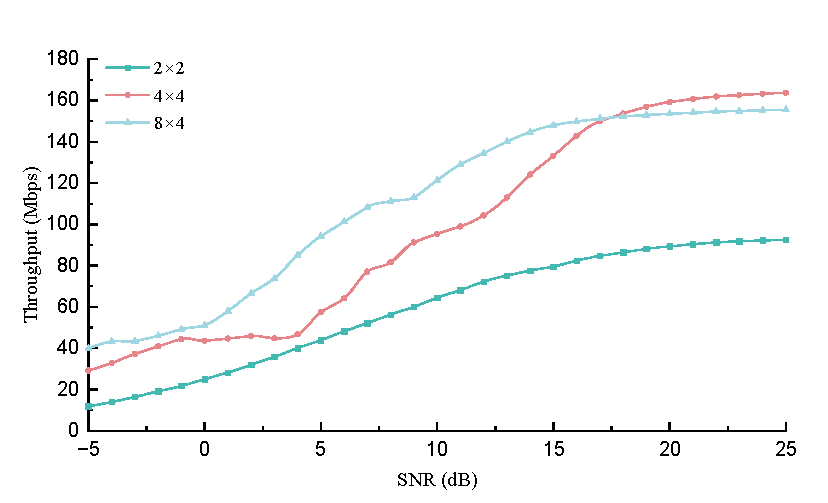
\includegraphics[width=0.75\linewidth]{figures/51AntennaNew.pdf}
			\caption{Downlink throughout performance under different MIMO configurations \hl{Still need to check 1x1 and 4x8 and 8x8? results}}
			\label{fig:51AntennaNew}
		\end{figure}
		
		\subsection{CDL Channel Profile Sweep}
		
		\begin{highlightblock}
		The second check varies the CDL channel profile while keeping the baseline $4\times4$ MIMO configuration and CSI feedback settings unchanged. 
		
		Figure~\ref{fig:52CDLBCD} compares the downlink throughput performance under CDL-B, a typical NLOS channel, and CDL-D, a typical LOS channel with the baseline. The CDL-C case corresponds to the baseline configuration.
	
		\end{highlightblock}
		
		\begin{figure}[H]
			\centering
			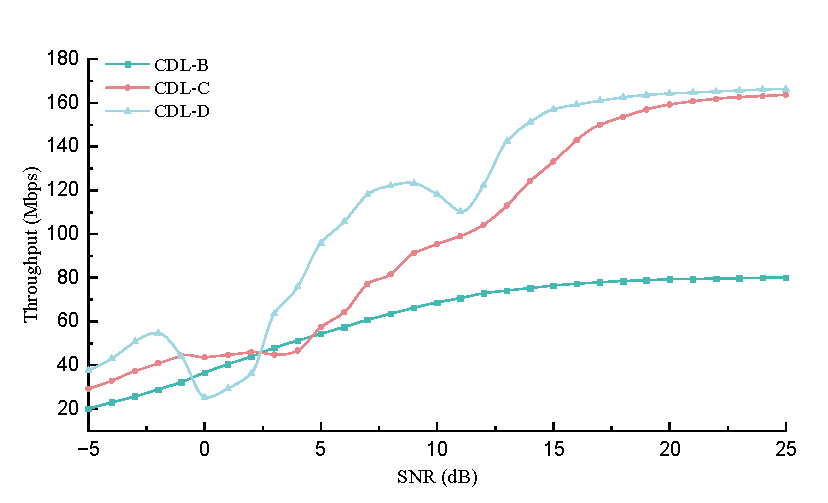
\includegraphics[width=0.75\linewidth]{figures/52CDLBCD.pdf}
			\caption{Downlink throughout performance under different CDL channel models}
			\label{fig:52CDLBCD}
		\end{figure}
		
		\begin{highlightblock}
			For all three CDL profiles, the throughput increases with SNR and eventually approaches saturated levels, showing that the general link-adaptation behaviour remains consistent. 
			
			However, the performance of the system under different channel models vary greatly. The CDL-B profile increases gradually, almost always worse than the baseline scenario and saturates at a much lower throughput, around 80 Mbps, as compared to baseline CDL-C. This is as expected as the CDL-B channel model has lower potential in spatial multiplexing as compared to CDL-C. <?>
			
			The CDL-D profile on the other hand achieves the best overall performance. It generally leads to higher throughput at low-to-medium SNR regions and, while leading to almost the same saturated throughput as CDL-C at the high SNR, enters the saturated zone in advance. The overall performance has approximately 5~dB in SNR gain as compared to the baseline. This behaviour is also as expected, as the CDL-D channel has a major LOS component, which supports reliable and rapid transmission even at a low SNR situation, leading to clear advantage as compared to other scenarios, when one-layer transmission is used.
			
			Overall, the CDL profile sweep shows that regardless the channel used, the overall shape of the throughput curve is to a large extent consistent. But the achievable throughput and required SNR are channel-dependent. For example, among the two additional models tested here, CDL-D mainly improves the transition-region SNR requirement while CDL-B represents a more limiting channel condition under the current setup <?>.
		\end{highlightblock}
		\subsection{One-layer Control Experiments}
		\label{sec:4.3}
		\begin{highlightblock}
			Similar to section \ref{sec:Fixed-rank}, a controlled experience  is conducted to test the performance of the simulations in this section performs when the maximum number of layers supported is fixed to 1, as shown in Figure~\ref{fig:53Fixed1Layer}. In contrast to the adaptive baseline, where the rank indicator is selected through CSI feedback, the transmission rank is constrained to one layer throughout the SNR sweep. 
			
			Considering the $4\times4$ cases, the conclusion from Fig. \ref{fig:52CDLBCD} remains mostly unchanged. CDL-B model is, across the whole simulated SNR range, largely worse than the baseline scenario. CDL-D channel outperforms the baseline at low-and-medium SNR regions, while achieving slightly lower saturated throughput than the baseline.
			
			Compared with the adaptive CDL profile sweep, the fixed one-layer result provides a useful diagnostic reference. In the adaptive case, performance differences may arise from both single-layer link quality and the ability of the channel to support spatial multiplexing. Under fixed one-layer transmission, however, rank adaptation is removed. Therefore, the remaining differences mainly reflect how each CDL profile supports robust single-layer transmission under the same CSI feedback and other configurations.
			
			Considering the sweep of MIMO configurations when the CDL-C channel model is used, the ....
		\end{highlightblock}
		\begin{figure}[H]
		\centering
		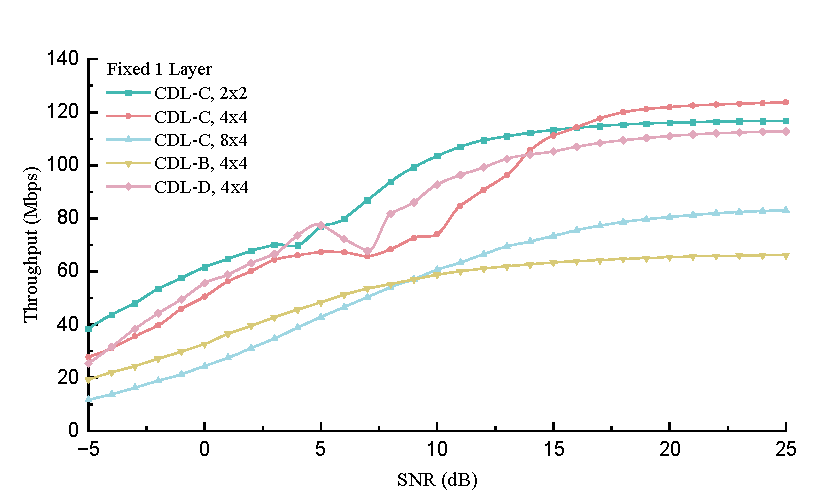
\includegraphics[width=0.75\linewidth]{figures/53Fixed1Layer.pdf}
		\caption{Downlink throughout comparison under fixed one-layer transmission \hl{Some issue with [2x2] and [8x4] curves, re-simulate}}
		\label{fig:53Fixed1Layer}
	\end{figure}
	
	
	
\section{Impact of Mobility and CSI Reporting Periodicity}
	\label{sec:5}
	
	\begin{highlightblock}
		This chapter investigates the impact of mobility and CSI reporting periodicity on the CSI-driven downlink transmission performance. In a time-varying channel, the CSI obtained from CSI-RS measurements may become outdated before it is applied for the transmission. This effect is expected to become more significant as the Doppler shift increases or as the CSI reporting period becomes longer. Therefore, this chapter first studies the impact of Doppler shift under the baseline scenario, before examining the effect of different reporting periodicities.
	\end{highlightblock}
	

		\subsection{Doppler Shift under Default CSI Reporting Period}
		\label{sec:5.1}
	\begin{highlightblock}
		Figure~\ref{fig:41Throughput_Speed} shows the impact of Doppler shift on downlink throughput under the baseline CSI reporting period. The three Doppler shifts, 10~Hz, 100~Hz, and 390~Hz, represent increasing levels of system mobility. With a carrier frequency of 3.5~GHz, these correspond approximately to UE speeds of 3~km/h, 30~km/h, and 120~km/h, respectively.
		
		The general throughput behaviour remains similar across all Doppler cases: the throughput increases with SNR, and eventually approaches a high-SNR saturation level. However, higher Doppler shift causes a visible rightward shift of the throughput curve. This indicates that, under higher mobility, a larger SNR is required to achieve the same throughput level.
	\end{highlightblock}

	\begin{figure}[H]
		\centering
		
\includegraphics[width=0.75\linewidth]{figures/41Throughput_Speed.pdf}
		\caption{Impact of Doppler shift on downlink throughput}
		\label{fig:41Throughput_Speed}
	\end{figure}


	\begin{table}[H]
		\centering
		\caption{Interpolated SNR values at selected target throughput levels}
		\label{tab:snr_interpolation}
		
		\begin{tabular}{cccc}
			\midrule
			\textbf{\makecell{Target Throughput\\(Mbps)}} & \textbf{\makecell{SNR 10 Hz \\(dB)}} & \textbf{\makecell{SNR 100 Hz \\(dB)}} & \textbf{\makecell{SNR 390 Hz \\(dB)}} \\
			\toprule
			50  & 4.3  & 5.5  & 6.7  \\
			80  & 7.7  & 8.9  & 10.5 \\
			110 & 12.7 & 12.7 & 14.4 \\
			140 & 15.7 & 16.2 & 17.9 \\
			\bottomrule
		\end{tabular}
		
		\vspace{0.3em}
		\raggedright
		\footnotesize{$^\dagger$ SNR values obtained using linear interpolation.}
		
	\end{table}
\begin{highlightblock}
		This observation is quantified in Table~\ref{tab:snr_interpolation}, which shows the required SNR level for each curve to reach different target throughput levels. The required SNR values are obtained by linear interpolation of the throughput curve. For example, to reach 80~Mbps, the required SNR increases from 7.7~dB at 10~Hz to 8.9~dB at 100~Hz and 10.5~dB at 390~Hz. This corresponds to an SNR penalty of approximately 1.2~dB and 2.8~dB relative to the 10~Hz baseline. Alternatively, with a target throughput of 140~Mbps, the 390~Hz case requires 17.9~dB compared with 15.7~dB for the 10~Hz case.
		
		At high SNR, the difference of throughput for different mobility cases become closer, although the higher-Doppler cases remain slightly lower. This suggests that high SNR can partially compensate for mobility-induced degradation. 
	\end{highlightblock}

		\begin{highlightblock}		
		The reason....................The degradation is consistent with CSI ageing. With a fixed CSI reporting period and processing delay, the CSI used for link adaptation becomes less representative of the actual channel at the time of transmission when the channel varies more rapidly. As a result, the selected RI, PMI, and CQI may become less accurate, leading to less effective precoding and MCS selection. The effect is most visible in the transition region, where link adaptation decisions are particularly sensitive to the estimated channel quality.???
		
		The results of this subsection motivate the following CSI periodicity study. Since the degradation at higher Doppler is partly caused by CSI ageing, reducing the CSI reporting period may help improve the freshness of the feedback and recover part of the throughput loss under high-mobility conditions.

\end{highlightblock}


	\subsection{Reporting Periodicity at Different Mobility}
	
	\label{sec:5.2}
		\begin{highlightblock}
			Following the observation from the previous subsection, figure~\ref{fig:42PO} compares the effect of CSI reporting periodicity under low- and high-mobility scenarios. In both cases, the CSI-RS and CSI reporting periods are varied simultaneously while the remaining configuration is kept unchanged, consistent with the baseline settings.
		\end{highlightblock}
				\begin{figure}[H]
				\centering
				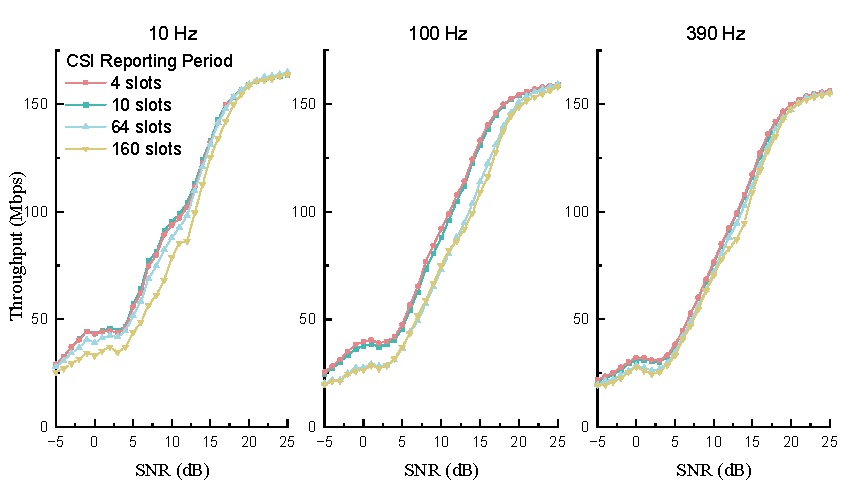
\includegraphics[width=\linewidth]{figures/42PO - Copy.pdf}
				\caption{Downlink throughput performance under different CSI reporting periods for low- and high-mobility scenarios}
				\label{fig:42PO}
				\end{figure}
		\begin{highlightblock}
			For the 10~Hz case, the throughput curves are relatively close across different reporting periods. For SNR below 20dB, the performance of low reporting periods 64 slots and 160 slots is clearly worse than the baseline performance, which is equivalent to a rightward shift of the throughput curve. As the SNR enters high region, the performance difference between different reporting periods converges, showing that the improvement in SNR can yield to ... The reporting per 4 slots however, does not in general show any noticeable improvement comparing to report every 10 slots.
			
			The observation shows that, even under low mobility where the channel changes slowly, having denser CSI remains useful, despite the throughput improvement is limited.
			
			For the high mobility 390~Hz case, similar trends has been observed. The 4-slot reporting period achieves the best performance for low-to-medium ranges, where longer periods require a higher SNR to reach similar throughput levels. At high SNR, the performance different shrinks and disappears. However, the amount of improvement clearly decrease compared to the low mobility scenario, which is unexpected and will be discussed in more following part.
			
			\hl {need to add 100Hz}
			
			Overall, the results show that reducing the CSI reporting period provides limited benefit under to the system. The main effect is an SNR gain in the transition region rather than a significant increase in high-SNR saturation throughput. 
			
			The CSI report also comes with the trade-off, despite having higher more frequent CSI improves the performance, it also increases uplink feedback overhead, impacting the uplink throughput and leading to higher UE processing and power consumption. Therefore, more detailed analysis will be conducted to quantify the benefit of having denser CSI report under different scenarios.
		\end{highlightblock}
			
		\begin{highlightblock}
				In the following analysis, a CSI reporting period of 10 slots is used as the baseline, denoted as \(P_0=10\). For each Doppler shift \(f_D\), the reference peak throughput is defined as
			\begin{equation}
				R^{\max}_{f_D}
				=
				\max_{\gamma} R_{f_D,P_0}(\gamma),
			\end{equation}
			where \(R_{f_D,P}(\gamma)\) is the measured downlink throughput at SNR \(\gamma\) under CSI reporting period \(P\). The target throughput level used for each mobility test case is 50\% of the reference peak throughput with 10 slots baseline reporting period. \\

			The SNR required for each reporting period $P$ with fixed mobility $f_D$ to reach the target throughput can be obtained by linear interpolation, denoted as $\gamma_{f_D,P}(0.5R^{\max}_{f_D})$. 
			
			The change in performance due to the use of different reporting period is evaluated base on the relative SNR penalty or gain with respect to the baseline
			\begin{equation}
				\Delta \gamma_{f_D,P}
				=
				\gamma_{f_D,P}(0.5R^{\max}_{f_D})
				-
				\gamma_{f_D,10}(0.5R^{\max}_{f_D}).
			\end{equation}
			Positive values of $\Delta \gamma_{f_D,P}$ indicate an SNR penalty, while negative values indicate an SNR gain. In addition to the slow and fast mobility scenarios tested from Fig. \ref{fig:42PO}, the medium mobility with 100~Hz Doppler shift is also tested. The quantitative results are shown in Table \ref{tab:csi_period_snr_required} below.
		\end{highlightblock}
		
		\begin{table}[H]
			\centering
			\caption{SNR required to reach 50\% of the baseline reference peak throughput}
			\label{tab:csi_period_snr_required}
			\begin{tabular}{llcc}
				\midrule
				\textbf{Doppler} & \textbf{CSI period} & \(\boldsymbol{\gamma}_{50\%}\) & \(\boldsymbol{\Delta\gamma}\) \\
				\toprule
				10 Hz  & 4 slots   & 8.2 dB & 0.1 dB \\
				10 Hz  & 10 slots  & 8.1 dB & -- \\
				10 Hz  & 64 slots  & 9.0 dB & 0.9 dB \\
				10 Hz  & 160 slots & 10.5 dB & 2.4 dB \\
				\midrule
				100 Hz & 4 slots   & 8.5 dB & -0.5 dB \\
				100 Hz & 10 slots  & 9.0 dB & -- \\
				100 Hz & 64 slots  & 11.0 dB & 2.0 dB \\
				100 Hz & 160 slots & 10.8 dB & 1.8 dB \\
				\midrule
				390 Hz & 4 slots   & 10.3 dB & -0.1 dB \\
				390 Hz & 10 slots  & 10.4 dB & -- \\
				390 Hz & 64 slots  & 10.8 dB & 0.4 dB \\
				390 Hz & 160 slots & 11.2 dB & 0.8 dB \\
				\bottomrule
			\end{tabular} \\
			$^\dagger$ Reference peak throughput values used: 
			163.9 Mbps at 10~Hz, 161.0 Mbps at 100~Hz, 158.0 Mbps at 390~Hz.
			
		\end{table}
		
		\begin{highlightblock}
			
			Table~\ref{tab:csi_period_snr_required} quantifies the relative impact of CSI reporting periodicity within each mobility condition.
			
			At 10~Hz, using very dense CSI reports have only a limited effect. The 4-slot and 10-slot cases require almost the same SNR to reach the target throughput, with only a 0.1~dB difference. However, increasing the reporting period to 64 and 160 slots introduces clear SNR penalties of 0.9~dB and 2.4~dB, respectively. This indicates that although the channel is slowly varying at 10~Hz, very infrequent CSI reporting can still degrade the performance at mid SNR region because the feedback becomes less representative of the current channel state.
		
	\end{highlightblock}
	\begin{highlightblock}
			For the 390~Hz case, consistent with the observation from Fig. \ref{fig:42PO}, having lower reporting period leads to penalties of  0.4~dB and 0.8~dB relative to the baseline, which is smaller than the penalty for 10~Hz scenario, which are 0.9~dB and 2.4~dB respectively. Increasing the report frequency to every four slots also only leads to ignorable amount of improvements. 
				
	\end{highlightblock}
	\begin{highlightblock}
			The impact of CSI period change has more visible impact for the 100~Hz scenario. The 4-slot case achieves a 0.5~dB SNR gain relative to the 10-slot baseline, showing that more frequent reporting does lead to better performance. In addition, slowing down the report to every 64-slot and 160-slot causes 2.0~dB and 1.8~dB additional SNR, respectively, much more dominant than the other two mobility scenarios.
		\end{highlightblock}
		
	\begin{highlightblock}
			The non-monotonic difference between 64 and 160 slots for the 390~Hz case and between 4 and 10 slots for the 10~Hz case should not be over-interpreted, as it is likely due to simulation inaccuracy, limited number of frames simulated, and the discrete nature of CSI-driven CQI, PMI, and RI decisions. 
			
			Overall, the results from this subsection show that CSI reporting periodicity mainly affects the SNR required in the transition region rather than the final saturation throughput. Shorter reporting periods can provide an SNR gain by reducing CSI ageing, especially under moderate mobility. Under low mobility (3km/h) case, having denser CSI period has only limited benefit to the transmission as the channel is not undergo rapid change. Under high mobility (120km/h) case, similar observation is observed, but the underlying reason is completely the opposite, since the channel is changing too-rapidly. Having short reporting period alone in this scenario does not fully recover the loss caused by rapid channel variation. The CSI is affected not only by the reporting period, but also by factors such as processing delay, channel estimation accuracy, and the time variation between CSI report and transmission, where these issues become especially dominant under high mobility.
			 
		\end{highlightblock}

	\subsection{Discussion of CSI Freshness and Practical Trade-Off}
		
	
	\begin{highlightblock}
		The results in Sections~\ref{sec:5.1} and~\ref{sec:5.2} show that the value of CSI feedback should not be evaluated only by its reporting granularity or reporting frequency. Instead, its effectiveness depends on the environment, especially the mobility of the system that impacts the channel directly. A visualization of the relative SNR offset under different situation is shown in Fig. \ref{fig:43lollipop} below based on data from Table \ref{tab:csi_period_snr_required}.
		
	\end{highlightblock}
	\begin{figure}[H]
		\centering
		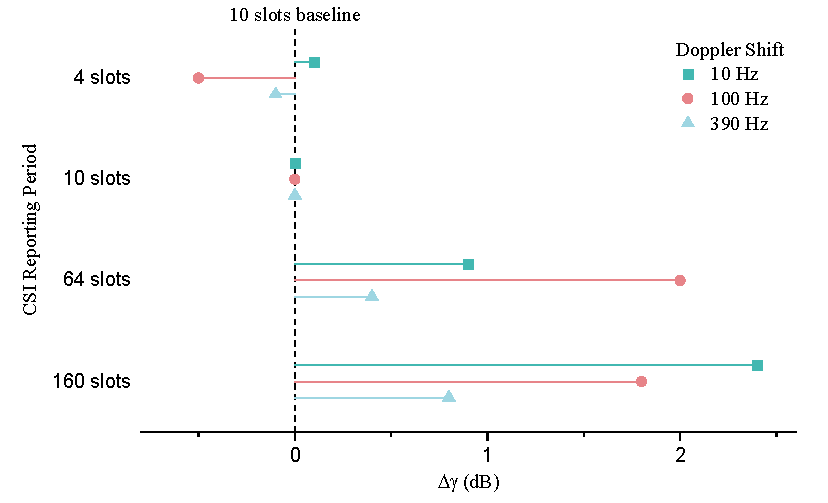
\includegraphics[width=\linewidth]{figures/43Lollipop.pdf}
		\caption{Relative SNR offset \(\Delta\gamma\) with respect to the 10-slot CSI reporting baseline}
		\label{fig:43lollipop}
	\end{figure}

	
	\begin{highlightblock}

		Based on the results, it is clear that a CSI reporting period is suitable to be used as the default setting during the transmission. It in general provides a satisfactory level of performance for the system while avoided the use of overly-frequent CSI reports. The 10 slots period is especially suitable as, for the 10~Hz and 100~Hz scenario, significant performance degradation will occur when the CSI period decreases from per 10 slots to 64 slots (0.9~dB and 2~dB respectively).
				\end{highlightblock}
		\begin{highlightblock}
		However, the results also shows that the system has the potential to adjust the CSI periodicity based on the channel condition, thus achieving a trade-off balance between the performance and the uplink throught as well as the UE power consumption. For example, when the UE is at medium-speed around 30~km/h, it has been proven that the system can enjoy a noticeable improvement in the throughput when increasing the reporting period from default baseline to per 4 slots. In the meantime, for high-speed scenarios such as on a train or motorway, using the default value may even be considered as a waste of energy for the UE. A CSI report every 64 slots, or options in between such as per 32 or 40 slots might be ideal. In addition, Fig. \ref{fig:42PO} has also showed that at high SNR, the throughput curves for different reporting periods converge to similar saturation levels. This suggests that having frequent CSI report is only beneficial at low-to-medium SNR regions. At high SNR regions, using per 64 slots or 160 slots reporting is already enough for the system.
		\end{highlightblock}
			\begin{highlightblock}
		More frequent CSI reporting improves the freshness of CSI and can reduce the SNR required to achieve a given throughput, but it also increases uplink feedback overhead and consumes more power of the UE. This overhead includes the resources required to transmit RI, PMI, and CQI reports, and becomes more significant when reporting is frequent. The observation here provides an insight to the CSI reporting period adjustment algorithm in terms of finding the most suitable reporting period based on the environment and channel status. 
				\end{highlightblock}
		\begin{highlightblock}
		Moreover, the simulation results suggest that the optimal CSI reporting period is mobility- and scenario-dependent. In addition to the fixed rules discussed in the previous paragraphs, a closed-loop feedback algorithm could be introduced during transmission to adaptively select the CSI reporting period. Starting from a default reporting period, or from an empirically selected value based on the current scenario, the system could adjust the reporting period among neighbouring options and measure the resulting gain or penalty. If the improvement is considered significant enough to justify the additional feedback overhead, the new CSI reporting period could be adopted for a predefined duration before being re-evaluated.
	\end{highlightblock}
	
	AI
	
	
	\newpage
	




\section{Discussion and Conclusion}
	\subsection{Interpretation of Results}
	\begin{highlightblock}
		
		The results from the previous sections confirm that CSI feedback functions as a meaningful link adaptation mechanism in the simulated 5G NR downlink system. 
		
		By allowing the transmitter to optimize rank, modulation scheme,  target code rate, and PMI according to the estimated channel condition, the system can avoid some inefficient fixed-transmission choices and therefore achieving better performance under given condition. The improvement due to CSI feedback is particularly clear from the fixed-rank control experiments in Section \ref{sec:3.4}, where constraining the rank leads to performance loss where the channel could otherwise support more adaptive transmission layer selections.
	\end{highlightblock}
	
	\begin{highlightblock}
		The robustness experiments from Section \ref{sec:4} further show that the overall behaviour of the system is universal and ......
		.... The result shows that different channel models antenna MIMO configurations lead towards similar behaviour of the throughput curves, despite the absolute values may vary largely depending on how the specific channel is constructed or the array and multiplexing gain brought by the MIMO system. 
	\end{highlightblock}
	
	\begin{highlightblock}
		In Section \ref{sec:5}, an in-depth investigation on the optimal selection of CSI reporting period based on the channel condition has been conducted. The results confirm that CSI freshness is a trade-off rather than an absolute objective. More frequent CSI reports can improve the accuracy of link adaptation noticeably when the channel varies sufficiently fast and when the system operates in a low-to-medium SNR region where the throughput curve is sensitive to CSI quality. However, once the system approaches the high-SNR saturation region, or when either the UE is nearly stationary or moving very fast, the extra feedback overhead may only bring limited downlink benefit, while leading to unnecessary power waste and reducing the maximum uplink throughput that can be achieved. A close-loop feedback algorithm for adaptive reporting period has also been proposed to balance between the trade-offs.
		
		Overall, the project shows that CSI feedback can greatly contributes to the performance of the downlink transmission. The reporting configuration should be set depending on the operating scenario, rather than being fixed purely by a conservative default value or simply targeting maximum possible downlink throughput.
	\end{highlightblock}
	
	\newpage
	\subsection{Limitations}
	\begin{highlightblock}
		The study is based on link-level simulation. Therefore, it focuses on the behaviour of a single downlink connection and does not explicitly model multi-user scheduling, MU-MIMO scenario, uplink transmission, traffic dynamics, or network-level resource allocation ?????. As a result, the conclusions are most directly applicable to physical-layer link adaptation rather than complete system-level network optimisation. Since only downlink is modeled, there is a lack of results on the quantitative cost of CSI reporting in terms of how the feedback overhead will lead to additional uplink resource consumption, therefore impacting the uplink throughput and UE power consumption. The trade-off between downlink throughput improvement and uplink reporting cost is therefore evaluated mainly from the observed downlink performance trends.
		
		In the meantime, the HARQ mechanism is disabled during the simulation for simplicity. Despite this would not lead to loss of generality, the absolute throughput in practice may deviate from the simulated ?????
	\end{highlightblock}
	
	\begin{highlightblock}
		The simulation uses a selected set of carrier, antenna, channel, Doppler and CSI-reporting configurations based on the default configuration commonly set during 3GPP requirement tests. These choices are sufficient to reveal the main trends, but they do not cover the full NR parameter space. Many other parameters, such as codebook types and CQI wideband versus subband settings or may lead to different quantitative results. 
	\end{highlightblock}
	
	\begin{highlightblock}
		Finally, despite practical factors such as the UE delay in CSI report processing has been considered during the simulation, the receiver and channel-estimation assumptions remain simplified compared with a real-life implementation. Practical hardware impairments, calibration errors, imperfect synchronisation and more are not fully represented. Therefore, the absolute throughput values should be interpreted as simulation-based indicators rather than direct predictions of field performance, and can generally be seen as the upper limit of the performance.
	\end{highlightblock}
	
	
	\subsection{Future Work}
	
	\begin{highlightblock}
		Future work could first introduce an explicit feedback-overhead model to quantify the cost of the CSI reporting period to the uplink. The proposed adaptive CSI reporting algorithm can be implemented and tested. This would turn the empirical observations in this project into a practical feedback-control strategy that can be implemented to the real-life system.
	\end{highlightblock}
	
	\begin{highlightblock}
		Further work could also extend the simulation to a wider range of deployment scenarios, including for different channel conditions and different antenna configurations. A system-level study that supports MU-MIMO would be useful for evaluating whether the link-level conclusions remain valid when resources are shared among multiple users, The adaptation algorithm is also expected to be more complicated when the base station is connected to multiple UEs.
	\end{highlightblock}
	
	\begin{highlightblock}
		Finally, due to the limited time, only a limited number of CSI settings have been investigated. Deeper CSI adaptive strategies can be investigated combining the effect of different settings under more diverse transmission conditions.
	\end{highlightblock}
	
	AI
	
	\subsection{Implications for 5G NR and Future Wireless Systems}
	\begin{highlightblock}
		The findings of this project have broader implications beyond the specific simulation cases considered in this report. Although the study is based on link-level simulation and cannot be seen as a direct prediction to the performance of the system in real-life testing conditions, it provides useful insights for standardisation-oriented discussions, especially for 3GPP,on the design and update of CSI standards. 
		
		In practical system design, the objective is not only to maximise downlink throughput, but also to balance downlink performance against uplink performance, UE power consumption, implementation complexity, compatibility and robustness under a range of vastly different conditions. Due to this, the simulated results suggest that overly frequent CSI reporting may not always be justified, especially when the resulting downlink throughput gain is limited or when the system already operates near the high-SNR saturation region. Therefore, an adaptive CSI reporting strategy as proposed may provide a more efficient solution than using a fixed configuration across all scenarios.
		
		The whole simulation is completed based on 5G NR. However, the 6G that is currently still under discussion and development have a lot in common with the 5G NR, including the CSI report. The trade-off is expected to become even more important in future 6G systems. Traditional mobile traffic has often been dominated by downlink services such as video streaming and content delivery. However, future applications may create stronger uplink demand, including high-resolution live streaming, extended-reality interaction, high volume data-exchange and so on In such scenarios, the uplink transmission will be as important as the downlink transmission, therefore aiming to have similar level of throughput. In this case the uplink resources will become increasingly valuable, and excessive CSI feedback may compete more frequently with user-data transmission. This further strengthens the need to evaluate CSI reporting and other related parameters.
		
		Overall, this project supports a broader design direction in which CSI feedback configuration should be selected according to scenario-dependent system utility. Rather than configure the CSI, such that peak DL throughput can be reached, future 5G and 6G systems could benefit from adaptive mechanisms that jointly consider channel variation, mobility, SNR region, and other factors such as the UL throughput and power consumption. This would allow CSI reporting to contribute to more efficient, robust and balanced wireless communication systems.
	\end{highlightblock}
\newpage
\section{References} \let\refname\relax
\thispagestyle{empty}
	\vspace*{-1cm}
	\begingroup
	\bibliography{FinalReport}
\endgroup

\newpage
\section{Appendix}
\thispagestyle{empty}
\subsection{Risk Assessment}
	A complete risk assessment was provided in the submitted Technical Milestone Report (TMR). Since this project is entirely simulation-based and does not involve any physical laboratory experiments, no safety-related or hardware-related risks were identified. The only practical risk identified was the limited time available for the project relative to the computational cost of the simulations.
	
	The risk assessment presented in the TMR remains valid, and the identified computational risk has been carefully managed throughout the project. For example, during the development of the simulation program, particular care was taken to ensure that the code could be executed in parallel on multiple CPU workers using the MATLAB Parallel Computing Toolbox, rather than being limited to a single CPU thread at a time. In addition, external computing resources were used where necessary, including the CUED central computing system \texttt{ts-access}.
	
\subsection{Ethical Statement}
	This project is entirely simulation-based and does not involve personal data or physical laboratory experiments. Therefore, no direct safety, privacy, or human-related ethical risks are identified. 
	
	From an environmental perspective, the project requires computational resources for MATLAB simulations. Although the total computational demand is very limited relative to most other simulation-based research projects, unnecessary computation was avoided where possible by using a consistent baseline setup, a clearly pre-defined experimental structure and an appropriate number of simulated frames to balance result accuracy and computational cost.
	
	Additionally, the findings of the project may have positive social and environmental implications, as they provide a detailed analysis of CSI feedback and MIMO techniques, which could potentially contribute to more efficient wireless communication system. For example, the results may help avoid using overly frequent uplink reporting when it is unnecessary. Improved link adaptation can also support better spectral efficiency and more reliable connectivity.
\subsection{Declaration of the use of generative AI}
	Generative AI tools, specifically ChatGPT and Google Gemini, were used in a limited capacity during the completion of the project. AI assistance was used mainly during the early stage of the project, including to facilitate the understanding of related concepts and to support the debugging of the MATLAB simulation implementation.  
		
	It can be confirmed that the experimental design, data analysis, interpretation of results, final conclusions, and report content were completed and verified by the author. No AI tool was used, in any form, to generate, modify, or manipulate the simulated data.
\newpage
\thispagestyle{empty}
\subsection{Detailed Baseline Simulation Configuration}


\begin{table}[H]
	\centering
	\caption{Baseline simulation parameters, adapted from TR 38.753 where applicable \cite{3GPPSimulationSpec}}
	\label{tab:appendix1}
	\begin{tabular}{|ll|c|}
		\hline
		\multicolumn{2}{|c|}{\textbf{Parameter}}                                                                                                                                   & \textbf{Value}               \\ \hline
		\multicolumn{2}{|l|}{Duplex mode}                                                                                                                                 & TDD                 \\ \hline
		\multicolumn{2}{|l|}{FR / Carrier frequency}                                                                                                                      & FR1, 3.5GHz         \\ \hline
		\multicolumn{2}{|l|}{Maximum Doppler shift}                                                                                                                                    &  10~Hz                  \\ \hline
		\multicolumn{2}{|l|}{Channel Bandwidth / SCS}                                                                                                                     & 40Mhz / 30kHz       \\ \hline
		\multicolumn{2}{|l|}{Maximum allowed rank}                                                                                                                                        & 4                   \\ \hline
		\multicolumn{2}{|l|}{Antenna configuration}                                                                                              & 4Tx4Rx              \\ \hline
		\multicolumn{2}{|l|}{Channel model}                                                                                                                               & CDL-C               \\ \hline
		\multicolumn{2}{|l|}{Delay spread}                                                                                                                               & 300~ns               \\ \hline
		\multicolumn{2}{|l|}{\begin{tabular}[c]{@{}l@{}}Codebook configuration \\ for PDSCH and DMRS\end{tabular}}                                                        & Single Panel Type I \\ \hline
		\multicolumn{2}{|l|}{MCS table}                                                                                                                               & Table 1 (64 QAM)               \\ \hline
		\multicolumn{1}{|l|}{\multirow{4}{*}{PDSCH configuration}}      & Mapping type                                                                                    & Type A              \\ \cline{2-3} 
		\multicolumn{1}{|l|}{}                                          & k0                                                                                              & 0                   \\ \cline{2-3} 
		\multicolumn{1}{|l|}{}                                          & Starting symbol                                                                                 & 2                   \\ \cline{2-3} 
		\multicolumn{1}{|l|}{}                                          & Length                                                                                          & 12                  \\ \hline
		\multicolumn{1}{|c|}{\multirow{4}{*}{PDSCH DMRS configuration}} & DMRS Type                                                                                       & Type 1              \\ \cline{2-3} 
		\multicolumn{1}{|c|}{}                                          & Number of additional DMRS                                                                       & 1                   \\ \cline{2-3} 
		\multicolumn{1}{|c|}{}                                          & \begin{tabular}[c]{@{}l@{}}Max. number of OFDM \\ symbols for DL front loaded DMRS\end{tabular} & 2                   \\ \hline

	\end{tabular}
\end{table}

% Please add the following required packages to your document preamble:
% \usepackage{multirow}
\begin{table}[H]
	\centering
	\caption{Baseline CSI simulation parameters, adapted from TR 38.753 where applicable \cite{3GPPSimulationSpec}}
	\label{tab:appendix2}
	\begin{tabular}{|ll|c|c|}
		\hline
		\multicolumn{2}{|c|}{\textbf{Parameter}}                                                                                                               & \textbf{Unit} & \textbf{Value}    \\ \hline
		\multicolumn{1}{|l|}{\multirow{5}{*}{\begin{tabular}[c]{@{}l@{}}NZP CSI-RS for \\ CSI acquisition\end{tabular}}} & CSI-RS resource type       &      & Periodic \\ \cline{2-4} 
		\multicolumn{1}{|l|}{}                                                                                           & Density                    &      & 1        \\ \cline{2-4} 
		
		\multicolumn{1}{|l|}{}                                                                                           & Symbol location                   &      & 4        \\  \cline{2-4} 
		\multicolumn{1}{|l|}{}                                                                                           & Subcarrier location                   &      & 0        \\ \cline{2-4} 
		
		\multicolumn{1}{|l|}{}                                                                                           & CSI-RS interval and offset & slot & 10, 1    \\ \hline
		\multicolumn{2}{|l|}{CQI}                                                                                                                     &      & Wideband \\ \hline
		\multicolumn{2}{|l|}{PMI}                                                                                                                     &      & Wideband \\ \hline
		\multicolumn{2}{|l|}{CQI/RI/PMI delay}                                                                                                        & ms   & 7        \\ \hline
	\end{tabular}
\end{table}


\subsection{Project Repository and Supporting Materials}
The simulation code and supporting materials developed for this project have been made available in a GitHub repository: \url{https://github.com/Bariumoxid/MIMOTechniques}. The repository includes the main MATLAB simulation scripts, configuration files, workflows, and representative test cases used to generate and validate the results presented in this report. It also contains additional supporting materials, including weekly progress reports, the logbook, and source files for the report and figures.


\end{document}
